\chapter{Theoretical Foundation}
\label{chap:theory}

The following chapter provides a theoretical foundation for the research conducted in this thesis. It introduces the basic concepts of material flow planning and simulation, digital twins, process mining, and verification, validation, and uncertainty quantification (\gls{vvuq}). The relevance of these concepts in the context of simulation-based digital twins and their application in corporate practice will also be discussed.


\section{Discrete Material Flow Systems and Simulation}
This section begins with an introduction of the underlying concepts of \gls{dmfs} and \gls{sbdt}.
\label{sec:material-flow}

\subsection{Basic Concepts}
\gls{dmfs} cannot be fully understood without first clarifying the principles of Discrete Event Simulation (\gls{des}) for Discrete Event Systems. In \gls{des}, a system changes its state through \textit{events} that occur at specific, discrete time instances. It is assumed that no changes occur between two successive events. Consequently, the state of the system is defined by the values of its descriptive variables at each event occurrence \autocite{varga2001discrete}. The time at which an event occurs is typically marked by a timestamp, and the scientific evaluation of such systems is conducted by analysing the discrete \textit{sequence} of events over time \autocite{robinson2014simulation}.

Simulation in this context refers to the process of imitating the operation of a Discrete Event System over time, often over the course of multiple event sequences and capturing it in a model. The core activities in a simulation involve constructing and experimenting with this model. A high-quality simulation abstracts the essential features of the system, which requires the modeller to have a sound a priori understanding of what `essential' means in the given context. Although the model can later be refined, its quality is primarily measured by its ability to predict outcomes and offer a diverse range of scenarios \autocite{maria1997introduction}.

When simulating \gls{dmfs}, their simulation describes the imitation of material flow systems by breaking down continuous flows into discrete events. Such material flow systems can be characterized as “systems processing discrete objects (parts) that move at regular or irregular intervals along transportation routes or conveyor lines, comprising production and logistic systems” \autocite{Arnold2006,Schwede2024}. These systems form the backbone of material flow planning and control structures. The central idea of material flow planning and control is to ensure that material requirements—both in terms of quantity and timing—are met during transportation and storage across the various stages of the supply chain \autocite{Gehr2007}. Importantly, the time horizon of interest spans from order placement up to delivery.

To summarize, \gls{dmfs} are often simulated using \gls{des}, which abstracts the continuous flow of materials into discrete events. The simulation is carried out using a model. The simulation and modeller are embedded in the context of material flow planning and control, which aims to ensure that material requirements are met across the supply chain. Successfully performed material flow planning and control induce high quality data for simulation and modelling purposes.

\subsection{Comparing DMFS}
\label{sec:comparing-dmfs}
Because the simulation of \gls{dmfs} often involves (discrete) event simulation, events in \gls{dmfs} need to be further differentiated to be comparable. \Textcite{Arnold2006} propose to differentiate \gls{dmfs} into static and dynamic components.

Static components describe the possible states of the system. Possible states can be the set of possible processes given a part or resource, for example. Dynamic components define the concrete material flow for a certain part or order.
Static components include parts, resources and processes \autocite{Schwede2024}. Parts are transformed by processes using resources, sometimes based on orders. Transformation can have an impact on physical properties of the parts (transformation model), spatial position (transition model), the quality of the parts (quality model) and takes time (time model) and uses resources (resource model). Resources have a capacity of handling parts in parallel (resource capacity model) and processes have a predecessor-successors relationship (process model).
Dynamic components are used to define the concrete dynamic material flow within the \gls{dmfs}. There are four components: Order generation, order control, resource control and supply control. Order generation defines the load the system must process. Order control defines how parts are processed, sometimes referred to as routing rules \autocite{mildeautomated}. Resource control defines how resources decide to handle processing requests, also sometimes referred to as priority rules. Supply control describes how supply parts are provided \autocite{mildeautomated,Schwede2024}.\footnote{Refer to the latter source for a more detailed description of the components.}


\subsection{Production Planning and Control}
\label{sec:ppc}
Successful companies use production planning and control frameworks to describe and optimize their \gls{dmfs}. After establishing a theoretical foundation and simulation approaches for \gls{dmfs}, this section thus focuses on \gls{ppc} as a critical factor influencing the quality and quantity of data generated by \gls{des}.
\gls{ppc} is the structured approach to planning, scheduling, controlling and managing all aspects of the manufacturing process. It involves the coordination of resources, processes, and orders to meet production goals. \gls{ppc} is essential for optimizing production processes, reducing costs, and improving quality. The main functions of \gls{ppc} include production planning, production scheduling, and production control. Production planning involves determining the production capacity, production goals, and production processes. Production scheduling involves creating a detailed schedule for production activities \autocite{kasper2024designing}. Production control involves monitoring and controlling production activities to ensure that production goals are met \autocite{kiran2019production}. Scheduling is usually the last step performed before execution of the plan \autocite{pinedo2012design}.

The integration of \gls{ppc} with simulation models is crucial, because it directly affects the data quality used in \gls{des} of \gls{dmfs}. Effective \gls{ppc} processes anticipate anomalies in the production cycle, allowing for adjustments that maintain system efficiency and reliability. If successful, these adjustments yield high-quality data that enhance the accuracy of simulation outcomes. \autocite{kiran2019production}.


\subsection{Key Performance Indicators}
\label{sec:relevant-kpis}
Up to this point, \gls{des} for \gls{sbdt} of \gls{dmfs} has been introduced, outlining the key factors that contribute to a robust simulation. A model differentiation framework proposed by \textcite*{Schwede2024} has been briefly presented to facilitate comparison of \gls{sbdt}. Furthermore, the critical role of \gls{ppc} in generating high-quality data for simulation has been discussed. These discussions ignored up until now that, even when \gls{sbdt} are integrated within well-functioning \gls{ppc} processes, various \gls{sbdt} models remain prone to errors and inherent trade-offs that must be addressed by the modeller \autocite{Tao2018ijamt}.

The goal conflict of the modeller when developing \gls{sbdt} can be described by the following conflict triangle in \autoref{fig:goals} \autocite{robinson2014simulation,balci2012life}.

\begin{figure}[htbp]
  \centering
  
\includegraphics[width=0.6\textwidth]{figures/goals.png}
  \caption[Conflict Triangle]{The goal conflict of the modeller when developing \gls{sbdt}. Aiming for higher accuracy often leads to higher computational costs and reduced scalability. Reduced computational cost often leads to reduced accuracy and scalability. Aiming for higher scalability often leads to reduced accuracy and  higher costs.}
  \label{fig:goals}
  \caption*{Illustration based on \autocite{robinson2014simulation,balci2012life}.}
\end{figure}

Focusing one of the three dimensions often leads to trade-offs in the other two dimensions. Oftentimes the data itself is not sufficient to decide on which goal to choose. Limited data points may hinder the modeller from reaching high validity. System architecture may block the system from reaching good scalability. Hardware limitations may hinder the modeller from reaching high efficiency.
At other times, corporate management may have a preference for one of the dimensions.

One solution to balance and quantify these goals can be achieved by defining a set of \gls{kpi}s. Some may already be available through \gls{ppc}, some may be calculated from \gls{des} data or the \gls{des} itself. Optimally, the data warehouse provides relevant views \autocite{cui2020manufacturing}. Because the \gls{sbdt} in theory mirrors the \gls{dmfs}, the KPIs gathered from \gls{ppc} and the \gls{des} should yield identical values. Deviations between the KPIs of the \gls{sbdt} and the \gls{dmfs} may indicate errors in the \gls{sbdt} or anomalies in the \gls{dfms}. The following KPIs are deemed relevant for the evaluation of \gls{sbdt} \autocite{friederich2023framework}:

\begin{equation}
  \text{Throughput} = \frac{\text{Number of units produced}}{\text{Time period}}
  \label{eq:throughput}
\end{equation}

\begin{equation}
  \text{Lead Time} = \text{End time of the process} - \text{Start time of the process}
  \label{eq:lead_time}
\end{equation}

\begin{equation}
  \text{Cycle Time} = \frac{\text{Total processing time}}{\text{Number of units produced}}
  \label{eq:cycle_time}
\end{equation}

\begin{equation}
  \text{Total Setup Time} = \sum_{i=1}^{n} \text{Setup Time}_i
  \label{eq:setup_time}
\end{equation}

The \gls{ppc} related KPIs may be provided by the above-mentioned data warehouse, because they are highly relevant in the context of production scheduling and control. \textit{Throughput}, as defined in \autoref{eq:throughput}, measures the number of produced parts at the last station in a specified period and is an indicator for the productivity of the manufacturing system \autocite{hopp2011factory, imseitif2019throughput}. \textit{Lead time}, formulated in \autoref{eq:lead_time}, is the cumulative time a part travels through the system from start to finish and serves as an indicator for the efficiency of the manufacturing system \autocite{slack2010operations, pfeiffer2016manufacturing}. \textit{Cycle time}, shown in \autoref{eq:cycle_time}, measures the same duration as lead time but focuses only on the active production process, excluding transports and waiting times \autocite{goldratt2004goal, griffin1993metrics}. \textit{Setup time}, as expressed in \autoref{eq:setup_time}, measures the time needed to prepare a machine for a new task and is an indicator for the flexibility of the manufacturing system \autocite{allahverdi1999review, allahverdi2008significance}. In the given use case, the thesis aggregates the setup time for all setup processes. All KPIs presented so far can be calculated dynamically when new data has been sent. Later on, they may serve as an alert system for the modeller to detect deviations between the \gls{sbdt} and the \gls{dmfs}, see \autoref{sec:vvuq-sbdt}.

\section{Digital Twin: Definition and Concepts}
\label{sec:digital-twin}
The latter section gave a short introduction into \gls{dfms}, \gls{des}, its metrics and the corporate processes accompanying the \gls{sbdt}. Now, the thesis sheds light on the \gls{dt} itself.

As introduced in the preceding chapter, \gls{dt} inherit the highest order of modelling fidelity compared to \gls{dm} or \gls{ds}. There are different definitions of \gls{dt} present in the literature \autocite{Negri2017promfg,zheng2019application,glaessgen2012digital,Demkovich2018def,boschert2016digital,grieves2014digital,kritzinger2018digital,Tao2018ijamt,zehnder2018representing}. Each of them highlights different aspects of the \gls{dt}. This thesis utilizes the definition by \textcite{grieves2014digital} which highlights the conceptual elements of the twin and its lifecycle focus:

\begin{quote}
  The digital twin concept (...) contains three main parts: A) Physical products in real space, (B) virtual products in virtual space and (C) the two-way connections of data and information that tie the virtual and real products together. \autocite{grieves2014digital}
\end{quote}

The physical product is the entity which is modelled. The virtual product represents the \gls{dt} itself, but also its infrastructure, for example data services making the real-time data flow possible \autocite{Tao2018ijamt}. The two-way connection is the data flow between the physical and the virtual product. The data flow is bidirectional. \textcite{zehnder2018representing} add that the data flow may contain meta data ``describing the data source and its context'.

\subsection*{Types of Digital Twins}
\label{sec:types-digital-twins}
Now that a unified understanding of \gls{dt} has been established, this section focuses on how \gls{dt} may be learned from different sources of information. The following list includes the most relevant types of \gls{dt}:

\begin{itemize}
  \item \gls{sbdt} \autocite{Lugaresi2021aifac,martinez2018automatic}
  \item \gls{dddt} \autocite{he2019data,Friederich2022}
  \item \gls{hdt} \autocite{luo2020hybrid,huang2023hybrid}
\end{itemize}


\gls{sbdt}s \autocite{Lugaresi2021aifac,martinez2018automatic,boschert2016digital} are based on \gls{des}. They utilize \gls{des} (see \autoref{sec:material-flow}) to create a dynamic representation of the physical system \autocite{schluse2016simulation,pantelides2013online}. To incorporate a \gls{sbdt} into workflows and processes, suitable data structures must be in place beforehand \autocite{boschert2016digital}. \gls{des} may improve the predictive capabilities of the model compared to manual twin creation. \gls{des} is able to model causal relationships between the events \autocite{francis2021towards}. In contrast, the development of a realistic simulation model requires experts and time \autocite{Charpentier2014}. If the simulation model fails to capture recent behaviour of the physical entity, a recalibration is mandatory \autocite{Friederich2022}. \gls{sbdt}s are improving the creation and updating processes of \gls{dt}s.

\gls{dddt} rely on the utilization of data to model the physical entity. The data may be gathered from sensors, data warehouses or other sources (later on developed framework summarizes this under the term data sources, see \autoref{sec:framework}). The data is used to train a model which represents the physical entity. The model may be a neural network, a decision tree or another \gls{ml} model. The model is then used to predict future states of the physical entity. The model may be updated with new data to increase its accuracy \autocite{he2019data,Friederich2022}. For a more detailed description of \gls{dddt} including its up- and downsides, see \autoref{sec:data-driven-digital-twins}.

\gls{hdt} combine different sources of information to create a more accurate model of the physical entity. The sources may be simulation models (see \autoref{sec:material-flow}), data-driven models (see \autoref{sec:data-driven-digital-twins}) or physics-based models. Physics-based models contain information about the physical properties and behaviours of the entity. They do not have to learn these characteristics from the data because this information is made available to the model \textit{a priori} \autocite{kapteyn2022data,aivaliotis2019methodology}. The simulation based models accompanying the physics-based one obeys characteristics of \gls{sbdt}, see above. The combination of different sources may make the \gls{hdt} more robust and a faster learner. \gls{hdt} unite the advantages of \gls{sbdt} with the knowledge advantage physics based models have. Unfortunately, they also inherit the disadvantages of \gls{sbdt} through their simulation character. Physics-based models may also involve heavy computational costs and domain expertise \autocite{kapteyn2022data}.

\subsection*{Data-Driven Digital Twins}
\label{sec:data-driven-digital-twins}

While \gls{sbdt}s and \gls{hdt} possess significant computational costs and require domain expertise, \gls{dddt} are able to learn from data without the need for a hand-written simulation model. The \gls{dddt} \textit{learns} the model. Learning in the context of \gls{dddt} is not trivial, several approaches have been proposed in the literature \autocite{he2019data,Friederich2022,francis2021towards}. Oftentimes, Data Science methods come to work. The learning process may be supervised or unsupervised. Supervised learning uses labelled data to train the model \autocite{cunningham2008supervised}. The label can symbolize different values of interest. Unsupervised learning uses unlabelled data to train the model \autocite{barlow1989unsupervised}. Oftentimes, the task at hand is to group the data into different categories, see \autoref{sec:knn} \autocite{Biesinger2019}.
The learning process may be online or offline. Offline learning uses the data \textit{once} for training, validation and testing, while online learning continuously updates the model with new data to adapt to changes in the physical system. Online learning is thus able to capture new trends in the data and to foresee concept drift \autocite{tsymbal2004problem}. \gls{dddt} have to be differentiated from data-driven simulation \autocite{Charpentier2014}, which involves human intervention to create highly individual solutions for the physical entity. The key difference is that every characteristic has to be explicitly described in the model by the expert, there are no efforts to let an intelligent algorithm learn these by itself. \gls{dddt} may be able to update themselves to new trends in the data by online learning, termed \textit{synchronization} \autocite{reinhardt2019survey}. Latter has to be differentiated from \textit{updating}, which is a manual process to take corrective action in the logic of the twin itself \autocite{Schwede2024}. An example for updating a \gls{dddt} may be the addition of a new feature to the model. An example for synchronization may be the adaption of the model to new trends in the data. The latter may be done by the model itself, the former has to be done by the modeller.
\gls{dddt}s thus rely less on domain expertise and manual model creation. A suitable model may be able to capture relevant trends in the data and to predict outcomes which describe most of the characteristics of the physical entity. \textcite{francis2021towards} propose several process steps a \gls{dddt} must undergo to be termed \textit{data-driven}:

\begin{enumerate}
  \item \textbf{Data Collection:} The relevant entities to be modelled have to be identified. This activity involves data gathering of the identified entities and ensuring a steady data stream to a database. The data may be gathered from sensors, data warehouses or other sources.
  \item \textbf{Data Validation:} This step involves cleaning and preprocessing the data. The data may contain missing values, outliers or other errors. The data has to be cleaned and preprocessed to ensure a high quality of the model. Plausibility checks may be performed to ensure the data is correct.
  \item \textbf{Knowledge Extraction:} After the data has been collected and cleaned, events have to be detected. \Citeauthor{francis2021towards} utilize process mining terms in this context, such as event detection and process discovery. The main goal in this step is to find a common ground on which events are of interest. The thesis later dives deeper into PM techniques applied here, see \autoref{sec:process-mining}.
  \item \textbf{(Semi-)automatic Simulation Modelling:} The data is used to train a model. The model is then used to predict future states of the physical entity. The model may be updated with new data to increase its accuracy.
  \item \textbf{Continuous Model Validation:} Interestingly, \citeauthor{francis2021towards} propose a continuous model validation. In the online learning case, they recommend to use the steady data stream to apply validation techniques continuously, see \autoref{sec:vvuq-sbdt}. The validation may be performed by comparing the model predictions with the real data. If the model deviates from the real data, the model may be recalibrated.
\end{enumerate}

\gls{dddt}s go one step further than \gls{sbdt} and minimize the influence of the human in the loop \autocite{francis2021towards,Friederich2022}. Faster model development and updating activities are the result. The third reason to automate \gls{dt} endeavours elaborated by \textcite{Schwede2024}, increasing prediction quality, rises and falls with the data quality, thus the gathering and preprocessing efforts of the modeller. Extrinsic factors like the number of data points available also play into the equation. If the number of features is greater than the number of samples, the curse of dimensionality hinders a good modelling performance \autocite{koppen2000curse}. \gls{dddt} should avoid biased or noisy predictions at all costs. The identification of \textit{relevant} events poses the risk of introducing a selection bias, rather a confirmation bias. The modeller may have the tendency to select events which complement his hypothesis. Random sampling may be a solution to this problem, but can destroy sequential information patterns in event sequences.

Overall \gls{dddt} are a promising approach to model the physical entity. If the right balance between human involvement and automated learning is found, it may be an efficient solution \autocite{francis2021towards}. Thinking one step ahead, employing data-based \gls{vvuq} approaches may also be a step forward. This topic will be discussed in Section \autoref{sec:ml-approaches}.

\label{par:asmg}
One last discipline, \gls{asmg}, is worth mentioning. \gls{asmg} has to be differentiated from \gls{dddt} by the effort to automatically generate models, not twins. \gls{dm} and \gls{ds} are the goal here, achieved with tools of \gls{des}. Automatic \gls{dt} generation is not necessarily the goal. It aims to automate the model generation process and tries to eliminate the human in the loop, \autocite{reinhardt2019survey,lechevalier2018methodology}. Automation is achieved by taking into account a diverse range of data sources, including Computer Aided Design data, PPS data, production manuals, process data and programming code, thus reaching a high data variability. The gathered data has to be processed online or offline as well through suitable frameworks or human intervention. Challenges lay in incomplete data \autocite{bergmann2014automatische}, although the same problems of \gls{dddt} also apply here. If the gained data is not mined thoroughly, human intervention is needed again, mitigating automation efforts.

To conclude this section about \gls{dt}, the thesis concludes that there are different types of \gls{dt} differentiated by their source of information retrieval. A lot of work has been done to make the \gls{dt} creation, updating and prediction process more efficient. By the help of simulation, data and automated model generation, the \gls{dt} may be created with less time and resources than manually.

\section{Process Mining and Event Logs}
\label{sec:process-mining}
After introducing the corporate embedding of \gls{dt}s and their types, the thesis now focuses on \gls{pm} and event logs. \gls{pm} is a discipline which aims to extract knowledge from event logs. Event logs are the data basis for \gls{pm}. The following section introduces the basic concepts of \gls{pm} and event logs.

\subsection{Core Concepts}
\label{sec:core-concepts}
\gls{pm} is a discipline established 1999 which is interdisciplinary rooted in the field of Data Science and Process Science \autocite{van2016data}. Data Science can be considered a process agnostic discipline \autocite{van2016data}, while process science uses models not covering hidden trends in the data. The bridge between both approaches is \gls{pm}. The goal of \gls{pm} is to use event data to identify and extract process information \autocite{vanderAalst2012}. This information is used to discover (process discovery), monitor (conformance checking) and improve processes (process enhancement \autocite{vanderAalst2012}) by using event logs. Such logs must contain a case ID, an activity name and a timestamp. Additional information like resource information, order information or other context information may be added to the log \autocite{vanderAalst2012}. Such logs assume that the process can be captured fully and sequentially.

\begin{table}[htbp]
  \centering
  \caption[Exemplary Event Log]{A fragment of a manufacturing event log: Each line corresponds to an event. The case ID groups unique events which are identified by an event ID to one group, a trace. The timestamp refers to the time of event occurrence, while the activity describes the event. In this example, additional information like resource name and cost are given as well. Case 1, for example, consists of five events, involving a warehouse, two inspectors, and one machine.}
  \label{tab:manufacturinglog}
  \resizebox{\textwidth}{!}{%
    \begin{tabular}{r r l l l r}
      \toprule
      \textbf{Case id} & \textbf{Event id} & \textbf{Timestamp} & \textbf{Activity}     & \textbf{Resource}  & \textbf{Cost} \\
      \midrule
      1                & 101               & 10-01-2025:08.00   & receive raw material  & Warehouse A        & 500           \\
                       & 102               & 10-01-2025:08.30   & initial quality check & Inspector Stefan   & 300           \\
                       & 103               & 10-01-2025:09.00   & cutting process       & Machine X          & 800           \\
                       & 104               & 10-01-2025:09.45   & assembly              & Worker Paul        & 600           \\
                       & 105               & 10-01-2025:10.30   & final inspection      & Inspector Eva      & 400           \\
      \midrule
      2                & 201               & 11-01-2025:07.45   & receive raw material  & Warehouse B        & 500           \\
                       & 202               & 11-01-2025:08.15   & cutting process       & Machine Y          & 800           \\
                       & 203               & 11-01-2025:09.00   & welding               & Robot Arm Z        & 700           \\
                       & 204               & 11-01-2025:09.45   & quality assurance     & Inspector David    & 400           \\
      \midrule
      3                & 301               & 12-01-2025:06.30   & receive raw material  & Warehouse C        & 500           \\
                       & 302               & 12-01-2025:07.00   & initial quality check & Inspector Claudius & 300           \\
                       & 303               & 12-01-2025:07.30   & CNC machining         & Machine W          & 900           \\
                       & 304               & 12-01-2025:08.15   & painting              & Worker Daniel      & 500           \\
                       & 305               & 12-01-2025:09.00   & packaging             & Worker Johannes    & 350           \\
      \bottomrule
    \end{tabular}%
  }
  \caption*{Own illustration based on \textcite{van2016data}.}
\end{table}

\autoref{tab:manufacturinglog} illustrates the \gls{pm} concepts. The case ID groups unique events which are identified by an event ID to one group, a trace. The timestamp refers to the time of event occurrence, while the activity describes the event. In this example, additional information like resource name and cost are given as well. Cases containing the same events identified by unique event IDs will have different case IDs \autocite{van2016data}. Process discovery may try to produce a process model from the event log. The challenge lies not in the recording of every trace present in the event log, rather in finding a generic representation of the most frequent traces. The process model must be generic enough to describe most traces, but specific enough not to get invalidated by future traces which may contain completely different events. Another major building block of this process model is accounting for trace concurrency. When several events may be identified to happen in parallel during the same time window, the model must recognize this, similar to a bias-variance trade-off lend from data science \autocite{briscoe2011conceptual}. The process must contain the most frequent traces but has to filter out traces which contain anomalies. Such anomalies like longer time per event due to a fire alarm have to be accounted for. Conformance checking may compare a given process model against a given event log. They are specialized in detecting aforementioned anomalies. A key insight in conformance checking lies in two possible deviations from reality: The given model does not capture the real behaviour or reality differs from the model. In the first case, the model is not working as intended. In the second case, the event log is corrupt. The third view on event logs, process enhancement, enables the modeller to use the generated process model to identify bottlenecks. Anomalies identified serve as a good starting point because they reveal errors in the process sequence. The given table offers costs associated to each event ID. This information may be used to create an event benchmark to further optimize the desired `ideal' trace.

More generally, \gls{pm} empowers the modeller to perform \gls{vvuq} of a process model, event log or described trace. This concept is captured by the terms \textit{Play-In}, \textit{Play-Out} and \textit{Replay} \autocite{damm2001lscs}, see \autoref{fig:playinoutreplay}.

\begin{figure}[htbp]
  \centering
  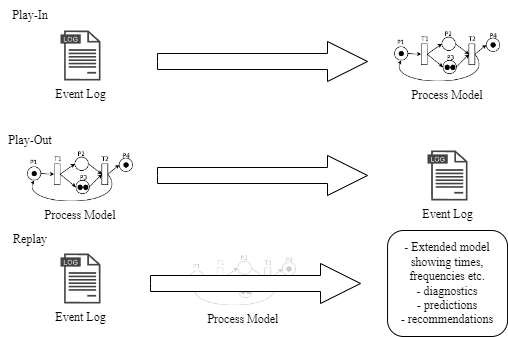
\includegraphics[width=0.8\textwidth]{figures/playinplayoutreplay.png}
  \caption[Process Model Usages]{The Play-In, Play-Out and Replay concept in the context of \gls{pm}. The Play-In phase involves the creation of a process model from an event log. The Play-Out phase involves the creation of an event log from a process model. The Replay phase involves the modification of the process model thorough information gained from the event log.}
  \label{fig:playinoutreplay}
  \caption*{Illustration based on \autocite{damm2001lscs}.}
\end{figure}

Play-In refers to the creation of a process model out of an event log. Play-Out may be called `sampling' in data science as it generates traces out of the model. \gls{des} uses Play-Out to generate new exemplary behaviour, see \autoref{sec:material-flow}. Here, a process model may be used to play-out (simulate) several traces of the desired events and then use bagging techniques like averaging the durations per event to gain robust KPIs (\autoref{sec:relevant-kpis}) and to reduce variance. A biased process model may still generate biased KPIs. Replay uses event log and process models together to check conformance, enriching the model with information captured in the log or to transform a descriptive process model into a prescriptive one \autocite{van2016data}.

\gls{pm} uses different formats to display process models like petri nets and BPMN models, among others \autocite{vanderAalst2012}. The thesis at hand focuses on \gls{dddt} in the context of simulation. Such data-driven models often involve complex inference steps not visible to the modeller \autoref{sec:requirements-automatically-generated-models}. Thus, they can not be rendered by \gls{pm} models which are transparent.

\subsection{Object-Centricness in Process Mining}
\label{sec:object-centric-event-logs}

The problem with traditional \gls{pm} lies in its single dimensionality of perspective. For each process analysis, a new play-out has to be performed. Interactions between different objects are not captured \autocite{van2023object}. One event may be related to different cases (convergence) or from the perspective of a case, there may be several equal activities within a case (divergence) \autocite{van2019object}.
Recently, \gls{oced} have been proposed as a new data basis for \gls{pm} \autocite{van2019object}. \gls{oced} logs (\gls{ocel}) are a generalization of classical event logs. Such traditional event logs use the case ID as a label to group and distinguish events. They assume that the process model describes the start and end of a single object. Each event refers to exactly one object (case) \autocite{van2023object}. \gls{oced} overthrows these assumptions by assuming that events may relate to multiple objects. To account for this new logic, \gls{ocel} coins the terms events, objects, types, attributes and qualifier. Each object has exactly one object type. Several objects may have the same type. An object type can be a description of the function such as machine, customer, supplier or activity descriptions such as invoice, request. Objects are instances of these types. Events in particular have an event type, termed activity. The same non-uniqueness applies here—many events can have the same type like ``processing complaint', ``cooking coffee'. Each event is described by exactly one type. \gls{oced} assumes event atomicity; each event is indivisible. Each event has one timestamp. Compared to traditional \gls{pm}, events may relate to multiple objects through a qualifier (event to order, E2O). Such a qualifier may be, considering the event ``printing label' and object ``printing station', the label to be printed. Objects may be related to multiple objects (order to order, O2O). O2O relationships are frozen (static) and are assumed to not change. The O2O relationship may be used to describe the order of producing a product. For example, the O2O relation ``main pcb to gyroscope' may say that the main pcb has to be produced before the gyroscope. Another O2O relation can be an order, the connection between the customer object and the ordered product. It is worth mentioning that objects can also be related indirectly together through two E2O relations: The E2O relation `producing' may connect the event ``machine 1 produces' with the object `gyroscope'. The E2O relation `check' may connect the event ``machine 1 checks' with the object ``main pcb', thus connecting the two objects `gyroscope' and ``main pcb' indirectly via two events \autocite{van2019object}. E2O relations are dynamic. They may change over time, involving different objects. In the given example, ``main pcb' would be checked with `display' instead of `gyroscope'.

Events and objects have attributes (keys), possessing values. Event attribute values refer to exactly one event and one event attribute; they are not shared. For example, the cost for one event may have the value $10€$. The same logic applies to objects as well, one event attribute value refers to exactly one object and one object attribute. Because several events may have the same type and several objects may have the same type as well, each event or object type may refer to any number of event or object attributes. They open interpretative possibilities for the modeller by considering them as expected attributes for the event or object type. The given example may be the event type `producing' which may have the event attribute `duration' and `cost'. The object type `gyroscope' may have the object attribute `weight' and `size'. One may average the different object attribute values of one type cluster to generate object type KPIs. A key specificity of object attribute values lies in the fact that they have a timestamp. Event attribute values do not. Latter information would be redundant because events do already have a timestamp, see above. Event attribute values may have cardinality one per event. $N$ event attributes have $n$ values. This does not apply to object attribute values. They may have multiple values because of their nature to change over time \autocite{van2023object}. This is why each object attribute value has a timestamp. The attribute value is in conclusion unique for a given object during a given time given one attribute. The given example may be the object attribute `weight' of the object ``main pcb' which may change over time. The object attribute value `weight' may have the value $100g$ at time $t_1$ and $120g$ at time $t_2$.

\gls{ocel} thus extends traditional \gls{pm} by accommodating the  multi-object nature of complex processes. Unlike classical event logs—which restrict events to a single case—\gls{ocel} captures dynamic interactions among multiple objects via E2O relations and static inter-object dependencies through O2O relations. This enriched framework enables a more comprehensive representation of real-world processes, where events may concurrently affect several objects. Timestamped object attribution values enable the modeller to perform temporal analysis and KPI derivation (\autoref{sec:relevant-kpis}). Overall, \gls{oced} provides a more detailed, semantically rich representation of complex, interconnected processes. \autocite{van2023object}.

\subsection{Process Mining as Enabling Technology}
\label{sec:process-mining-enabling-technology}

\gls{pm} uses event logs to develop process models or to enhance existing ones, so these logs may serve as a foundation for \gls{vvuq} of models in general. Live twin data often can be exported to the event log format. Several standardizations have been proposed, with the IEEE XES standard being the most widely used \autocite{van2016data}. The XES standard defines a common format for event logs, enabling the exchange of event data between different software frameworks. The idea lies in exporting twin decisions or live data as event logs and then use \gls{pm} tools to perform \gls{vvuq}.
Replay may be used on \gls{sbdt} simulated traces in comparison with actual event data to reveal mismatches in sequences or timing. For example, the \gls{sbdt} could have predicted a circular process. Replay can be applied to further analyse this bottleneck. Play-Out can empower the modeller to sample a big amount of exemplary traces to gain KPIs. \gls{oced} object attribute values may offer even more insights.
\gls{ppc} systems (\autoref{sec:ppc}) often times deliver even more data to enrich the event log so that \gls{vvuq} can be performed easier. If event log extraction out of the \gls{sbdt} is performed online, \gls{vvuq} can be performed on the fly. Both sources of information are incorporated in the framework, see \autoref{sec:framework}.

\section{VVUQ in the Context of Simulation-Based Digital Twins}
\label{sec:vvuq-sbdt}

The previous sections introduced the concepts of \gls{des}, \gls{ppc}, relevant KPIs, \gls{dt}, \gls{pm} and \gls{oced}. This section now focuses on \gls{vvuq} in the context of \gls{sbdt}. The thesis at hand uses the term \gls{vvuq} to describe the process of verifying, validating and quantifying the uncertainty of a \gls{sbdt}. V\&V has a long history in manufacturing and \gls{des} \autocite{Bitencourt2023}. \Textcite{sel2025survey} add uncertainty quantification as a main interest. Their framework is applied in the medical domain, but they mention reasonable arguments regarding efficiency and safety of \gls{sbdt} in general.\footnote{To go into detail, they deem erroneous data through sensor failure, model opacity (\autoref{sec:requirements-automatically-generated-models}) and the speed of model self-adaption as the necessities for UQ.} Thus, the thesis considers \gls{vvuq} instead of merely V\&V efforts. The following section introduces the basic concepts of \gls{vvuq} and its relevance for \gls{sbdt}.


\subsection{Development Process of VVUQ Concepts}
\label{sec:historical-development}
With the uprising of simulation models in the early 1950s \autocite{evans1967simulation}, the need for \gls{vvuq} arose unknowingly to the modellers. The usability of such simulations was deemed high as long as the results were promising, increasing trust in the technology \autocite{durst2017historical}. Blind trust does not validate models. Contrarily, if the results more or less were satisfactory, the model was considered validated \autocite{bonani2003physics}.

The first effort to define and perform verification was performed by \textcite{machlup1955problem} defining verification as ``including the correctness of mathematical and logical arguments, the applicability of formulas and equations (...), the reliability and exactness of observations, the reproducibility of experiments, the explanatory or predictive value of generalizations.''. \Textcite{naylor1967verification} further refined this definitions by introducing the idea of ``goodness of fit'. Latter describes the capability of the model to correctly reflect the modelled system. During the 1970s, researchers like \textcite{schlesinger1979terminology} defined validation as achieving a ``satisfactory range of accuracy consistent with the application', while Ignall argued for validation against simulations rather than analytical models \autocite{ignall1978using}. Sargent's work from 1979 to 1984 proposed methods like user collaboration and independent verification and validation (V\&V), detailing techniques such as sensitivity analysis and Turing tests \autocite{Sargent2010wsc}. Balci developed a taxonomy and emphasized continuous V\&V, reflecting the need for ongoing assessment \autocite{balci2012life}.

By 2004, modern V\&V emerged. Considering model fidelity of todays approaches, \textcite{Oberkampf2004amr} introduced widely recognized definitions of V\&V:

\begin{quote}
  \textit{Verification} is the process of determining that a model implementation accurately represents the developer's conceptual description of the model and the solution to the model.

  \textit{Validation} is the process of determining the degree to which a model is an accurate representation of the real world from the perspective of the intended uses of the model. \autocite{Oberkampf2004amr}
\end{quote}

Verification thus concerns itself with the \textit{correctness} of the given model \autocite{Sargent2010wsc}, while validation evaluates the \textit{quality} of explanations quantitively \autocite{Oberkampf2004amr}. \Textcite{iso2017systems} span the concept of validation to computational models, where valid models correctly reflect the users intended functionality. \gls{ppc} may provide the modeller with relevant KPIs to assess both.

\label{sec:uncertainty-quantification}
Uncertainty quantification (UQ) is a relatively new field in V\&V. It aims to quantify the uncertainty of the model and its predictions through the whole lifecycle of the model, including training, inference and prediction \autocite{sel2025survey}. UQ empowers the modeller to define confidence intervals to correctly emphasize the stochastic nature of the model predictions \autocite{volodina2021importance}. This is crucial for \gls{sbdt}, where real-time decisions rely on accurate representations, as \textcite{francis2021towards} highlights the need for continuous updates. UQ differentiates \textit{aleatory} uncertainty, which is inherent to the data, and \textit{epistemic} uncertainty, which is due to lack of knowledge \autocite{sel2025survey}. Aleatory uncertainty may arise due to sensor errors in the physical entity, generating noise. Epistemic uncertainty may arise due to lack of data or knowledge about the physical entity \autocite{thelen2023comprehensive}. Epistemic uncertainty can be reduced. \Textcite{abdoune2022handling} list UQ challenges and potential solutions in the context of \gls{sbdt}.

For \gls{sbdt}, \gls{vvuq} is not a one-time activity but rather a continuous process (\autoref{sec:framework}), ensuring \gls{dt} mirror physical systems accurately. This is important for industries like manufacturing, where decisions based on \gls{dt} have significant implications \autoref{sec:problem}.
The historical development of \gls{vvuq}, from early verification to integrated UQ, reflects the growing complexity of simulation models. As \gls{sbdt} become central to decision-making, robust \gls{vvuq} practices ensure reliability, linking back to foundational concepts introduced earlier, see \autoref{sec:types-digital-twins}. The concepts of \gls{vvuq} are embedded in the context of \gls{pm} and \gls{oced}, which may further assist described endeavours. Especially for UQ, \gls{pm} offers a rich data source to quantify uncertainty and validate models by providing a \textit{degree of fit} of the given process model.


\subsection{VVUQ for Automatically Generated Models}
\label{sec:requirements-automatically-generated-models}
Automatically generated models largely stem from the \gls{des} discipline (\autoref{par:asmg}), termed automatic simulation model generation, \gls{asmg} \autocite{mildeautomated,Charpentier2014}. They may use data-driven techniques which reduce the manual effort to create and update themselves. These models adapt quickly to changing conditions, making them valuable for dynamic environments like manufacturing. However, ensuring their reliability requires specific \gls{vvuq}. Because \gls{asmg} models often are black boxes, traditional \gls{vvuq} methods may not be applicable. The challenge lies in understanding the models internal logic and ensuring it accurately reflects the physical system. If sophisticated data driven methods have been applied, several \textit{key challenges} arise, hindering successful \gls{vvuq}:

\begin{itemize}
  \item \textbf{Model Opacity:} \gls{asmg} models often use complex \gls{ml} algorithms like neural networks. Such blackbox models are difficult to interpret, making it hard to understand their internal logic. This opacity may hinder \gls{vvuq}, as the modeller cannot easily identify errors or biases.
  \item \textbf{Data Dependency:} Data-driven models rely on high-quality data. If the data is biased or noisy, the models predictions may be inaccurate.
  \item \textbf{Dynamic Model Adaptation:} Models that continuously learn and adapt, such as those using online learning, require ongoing validation to ensure they remain valid as new data is ingested. This dynamic nature introduces the risk of concept drift \autocite{lu2018learning}, where the underlying process changes over time, potentially degrading model performance.
  \item \textbf{Quantifying Uncertainty:} Model predictions are stochastic in nature. For applications where precision is crucial, such as in manufacturing, uncertainty needs to be quantified.
\end{itemize}

To assess these challenges, the thesis defines the following \textit{key requirements} for \gls{vvuq} of automatically generated models, especially \gls{sbdt}:
\begin{itemize}
  \label{par:key-requirements}
  \item \textbf{Model Interpretability:} \label{par:surrogate} Models should be interpretable to ensure the models internal logic is transparent and understandable, enabling the modeller to identify errors or biases. Developing and employing techniques to make the decision-making processes of automatically generated models more transparent is crucial for \gls{vvuq}.
  \item \textbf{Upholding Data Quality:} Procedures to ensure that the data used for model generation and validation is accurate, complete, and representative of the operational environment are important. This includes data cleaning, preprocessing, and plausibility checks to identify and mitigate issues like missing values, outliers, or biases. For instance, in manufacturing digital twins, sensor data must be validated for accuracy and consistency to ensure reliable model outputs \autocite{rodriguez2023updating}.
  \item \textbf{Validatable Algorithms:} Besides ensuring model interpretability, the algorithms used for model generation must be validatable.
  \item \textbf{Continuous Validation:} \gls{vvuq} processes have to work in real-time to ensure the model remains valid as new data is ingested. This requires continuous monitoring and validation of the models predictions against real-world data. Techniques like online validation \autocite{francis2021towards} can help ensure the models accuracy and reliability over time.
  \item \textbf{Integration:} \gls{vvuq} processes have to be integrated into existing model- and \gls{ppc} infrastructure to be able to perform \gls{vvuq} on the fly. This requires close collaboration between data scientists, domain experts, and IT specialists to ensure the integration of \gls{vvuq} processes into the model lifecycle.
  \item \textbf{Scalability:} \gls{vvuq} processes have to be scalable as the underlying model or data evolves over time.
\end{itemize}

As noted by \textcite{francis2021towards}, the lifecycle \gls{sbdt} has implications for its \gls{vvuq} as well: \gls{vvuq} must accompany the \gls{sbdt} in all phases, from conceptualization to deployment and operation. The key requirements outlined above provide a foundation for developing robust \gls{vvuq} processes for automatically generated models.

\subsection{Traditional versus Machine Learning-Based Approaches}
\label{sec:ml-approaches}

\gls{vvuq} can be performed using traditional methods or more sophisticated approaches. Traditional verification techniques may include code inspection, unit testing or debugging \autocite{maniaci2018verification}. If closed solutions to simulated models are available, they may be used to validate the simulation. Traditional validation techniques involve comparisons between model predictions and real-world data, such as statistical tests or sensitivity analysis. In the context of manufacturing, simple experiments or historical data can be used. The consultation of experts is another possibility \autocite{shao2023credibility}.

\subsubsection*{Machine Learning-Based VVUQ}

Sophisticated approaches may include the use of \gls{ml} techniques to enhance \gls{vvuq} processes. ML can be used to identify patterns in data, detect anomalies, and improve model predictions. In addition to supervised and unsupervised learning shortly introduced in \autoref{sec:data-driven-digital-twins}, semi-supervised learning and reinforcement learning are two other approaches. Supervised learning may be used where labels regarding the validity or non-validity of an \gls{ocel} (see \autoref{sec:object-centric-event-logs}) are given. Unsupervised learning may provide such labels as learned categories if they are missing or may assist with finding common patterns in the data. Unsupervised techniques are context-agnostic and assume no patterns in the data, see \textcite{hastie2009unsupervised}. Semi-supervised learning combines labelled and unlabelled data to improve model performance. It somehow forms a middle ground where lots of unlabelled data is available and is then grouped by the algorithm. The scarce data is then used in the holdout set to perform testing \autocite{learning2006semi}. Reinforcement learning is not commonly applied in \gls{vvuq} of \gls{sbdt}.
ML techniques are often referred to as `oracles' when used for \gls{vvuq} because of their key challenge of opacity, \autoref{sec:requirements-automatically-generated-models}.

\subsubsection*{Challenges in Data Preparation and Feature Selection}

Before discussing the application of ML techniques in \gls{vvuq}, several problems hindering successful application of ML in \gls{vvuq} are identified. The first problem is data quality \autocite{wu2025uncertainty}. Data quality may degrade the performance and reliability of ML-based \gls{vvuq} approaches. Firstly, \textit{missing values} in the dataset can hinder the training process and potentially introduce biases. To account for this, imputation strategies or simply removing defect rows may be a solution \autocite{gudivada2017data}. The modeller has to keep in mind that this may corrupt the \gls{vvuq} process. Secondly \textit{outliers}, which are data points that deviate significantly from the rest, create a challenge as they might represent real trends in the data (and thus containing valuable edge cases for \gls{vvuq}) or simply be erroneous entries, requiring care from the modeller. Thirdly \textit{noise} can superimpose the underlying patterns that ML algorithms aim to learn, reducing the accuracy and generalization ability of the \gls{vvuq} models \autocite{liu2020noise}. Such noise may be random, for example by measuring environmental influence, or systematic, for example emitted by erroneous sensors. The first kind of noise can be reduced by smoothing or filtering.

Inconsistent data is another mistake to avoid in data gathering. It may arise from deviations in formats, units or representations of the same information. It can lead to confusion for ML algorithms and require standardization and cleaning \autocite{mahanthappa2021data}. Duplicate data entries may also generate false trends in the data. Imbalance introduced by duplicates or measurement errors can bias the model in predicting only the majority class when a classification problem is at hand.
Beyond data quality, the modeller has to make sure that the data is representative and bias-free. The training data used for \gls{vvuq} models must accurately reflect the environment. Biases can arise through human intervention or environmental influence \autocite{liu2020noise}. Finally, the way data is split into training, testing, and validation sets is important for avoiding overfitting, where the model memorizes the training data and fails to generalize to unseen data.

After ensuring data quality, the modeller has to consider suitable features for the given problem. Features are columns in the dataset describing characteristics of the data points (rows) through values. \gls{ocel} provide a relatively strict feature set in which the modeller has to operate. This has the advantage that several of the upper challenges may be eliminated because the data can be exported through a standardized interface. Successful \gls{vvuq} methods may require additional features nonetheless. Only the most relevant features may be selected \autocite{geron2022hands}. Feature engineering describes the endeavour of creating new features through combining existing features or through a new data gathering process. The incorporation of features in model training is coined feature selection. In the given use case, an adaptive feature a feature selection based on twin components may be useful, see \autoref{sec:comparing-dmfs}.

\subsubsection*{Classification Methods for the Detection of Model Deviations}
\label{sec:classification-methods}
Extensive work has been done on the topic of ML-based deviation detection. Such deviations are called `anomalies' and the process is termed ``anomaly detection' \autocite{kharitonov2022comparative}. Anomalies are data points that deviate significantly from the majority of the data. They can be classified into three categories: point anomalies, contextual anomalies and collective anomalies \autocite{chandola2009anomaly}. Point anomalies are single data points that differ significantly from the rest of the dataset. Contextual anomalies are data points that are normal in one context but anomalous in another. They appear less often than point anomalies and have less statistical weight. Collective anomalies are groups of data points that are anomalous when considered together but may not be anomalous individually. Anomalies are of special interest in the context of \gls{vvuq}, as they can indicate potential issues with the model or the data, see \autoref{sec:relevant-kpis}.

Anomaly detection and \gls{vvuq} share common goals of identifying deviations from expected behaviour and ensuring the reliability of models. The two fields can benefit from each other, as \gls{vvuq} can provide a framework for evaluating the performance of anomaly detection algorithms, while anomaly detection techniques can enhance \gls{vvuq} processes by identifying potential issues in models or data.
Several algorithms exist to detect anomalies, including statistical methods, clustering-based methods, and supervised learning methods. If the data is sufficiently labelled and preprocessed, supervised methods are promising. Algorithms such as Support Vector Machines (SVM), Neural Networks (NN), Decision Trees, and Random Forests can learn from this labelled data to classify new model outputs or behaviours as either normal or divergent. However, a common challenge in anomaly detection scenarios is the issue of class imbalance, where instances of normal behaviour are more common than the occurrences of deviations. This imbalance needs to be carefully addressed during model training to prevent the classifier from being biased towards the majority class. Clustering-based unsupervised methods detect anomalies through grouping similar data points together. Algorithms like K-Means, DBSCAN, and Hierarchical Clustering can be used to identify clusters of normal behaviour, with anomalies being those points that do not belong to any cluster. They measure the distance between data points to cull anomalous points as reaching far outside of a group of common data points. Oftentimes the assigned groups can be plotted, yielding further insights in the nature of the detected anomalies. Statistical methods, on the other hand, rely on the assumption that the data follows a certain distribution. They identify anomalies based on statistical properties such as mean, variance, and standard deviation \autocite{chandola2009anomaly}.

\subsubsection*{Metrics for Model Quality Measurement}
\label{sec:metrics-theory}
Another important aspects of assessing model quality is through metrics. The following section introduces the most common metrics used in \gls{vvuq} of \gls{sbdt}. The introduction is supported by an exemplary \gls{ocel}:

\begin{table}[H]
  \centering
  \caption[Exemplary OCEL]{A fragment of a manufacturing \gls{ocel} with type annotations. Each row represents an event with associated process execution details. The columns are annotated as follows: \texttt{process\_execution\_id} (int), \texttt{order\_id} (int), \texttt{start\_time} (datetime), \texttt{end\_time} (datetime), \texttt{part\_id} (int), \texttt{process\_type} (int), \texttt{process\_id} (int), \texttt{resource\_id} (int), and \texttt{is\_valid} (bool).}
  \label{tab:exemplary-ocel}
  \resizebox{\textwidth}{!}{%
    \begin{tabular}{r r l l r r r r l}
      \toprule
      \textbf{process\_execution\_id} & \textbf{order\_id} & \textbf{start\_time} & \textbf{end\_time}  & \textbf{part\_id} & \textbf{process\_type} & \textbf{process\_id} & \textbf{resource\_id} & \textbf{is\_valid} \\
      \midrule
      0                               & 2529               & 2020-04-22 14:21:07  & 2020-04-22 14:21:31 & -1                & 0                      & 0                    & 0                     & True               \\
      1                               & 2529               & 2020-04-22 14:23:35  & 2020-04-22 14:23:58 & -1                & 1                      & 1                    & 1                     & True               \\
      2                               & 2529               & 2020-04-22 14:21:09  & 2020-04-22 14:21:33 & -1                & 0                      & 0                    & 0                     & True               \\
      3                               & 2529               & 2020-04-22 14:23:36  & 2020-04-22 14:23:58 & -1                & 1                      & 1                    & 1                     & True               \\
      4                               & 2529               & 2020-04-22 14:21:11  & 2020-04-22 14:21:35 & -1                & 0                      & 0                    & 0                     & True               \\
      5                               & 2529               & 2020-04-22 14:23:36  & 2020-04-22 14:23:58 & -1                & 1                      & 1                    & 1                     & True               \\
      6                               & 2529               & 2020-04-22 14:21:13  & 2020-04-22 14:21:37 & -1                & 0                      & 0                    & 0                     & True               \\
      7                               & 2529               & 2020-04-22 14:23:36  & 2020-04-22 14:23:58 & -1                & 1                      & 1                    & 1                     & True               \\
      8                               & 2529               & 2020-04-22 14:21:15  & 2020-04-22 14:21:39 & -1                & 0                      & 0                    & 0                     & True               \\
      9                               & 2529               & 2020-04-22 14:23:37  & 2020-04-22 14:23:58 & -1                & 1                      & 1                    & 1                     & True               \\
      10                              & 2529               & 2020-04-22 14:21:18  & 2020-04-22 14:21:41 & -1                & 0                      & 0                    & 0                     & True               \\
      11                              & 2529               & 2020-04-22 14:23:37  & 2020-04-22 14:23:57 & -1                & 1                      & 1                    & 1                     & False              \\
      12                              & 2529               & 2020-04-22 14:21:20  & 2020-04-22 14:21:44 & -1                & 0                      & 0                    & 0                     & False              \\
      13                              & 2529               & 2020-04-22 14:23:37  & 2020-04-22 14:23:57 & -1                & 1                      & 1                    & 1                     & False              \\
      14                              & 2529               & 2020-04-22 14:21:22  & 2020-04-22 14:21:46 & -1                & 0                      & 0                    & 0                     & False              \\
      15                              & 2529               & 2020-04-22 14:23:38  & 2020-04-22 14:23:57 & -1                & 1                      & 1                    & 1                     & False              \\
      \bottomrule
    \end{tabular}%
  }
  \caption*{Tabulation based IoT Factory data.}}
\end{table}

\paragraph{\textbf{Accuracy}}
Accuracy measures the overall correctness of the classification model. It represents the ratio of correctly classified instances to the total number of instances in the dataset \autocite{fahrmeir2016statistik}.


\begin{equation}
  \label{eq:accuracy}
  \text{Accuracy} = \frac{\text{Number of Correct Predictions}}{\text{Total Number of Predictions}} = \frac{TP + TN}{TP + TN + FP + FN}
\end{equation}
where $TP$ denotes the count of true positives, $TN$ represents true negatives, $FP$ shows false positives, and $FN$ indicates false negatives.

This metric offers a high-level overview of the models performance by showing the proportion of predictions that align with the actual classes. Accuracy may be a misleading metric when dealing with imbalanced datasets \autocite{fahrmeir2016statistik}. In manufacturing, where the occurrence of invalid processes might be significantly lower than valid ones, a high accuracy score could be achieved by a model that often predicts the majority class, failing to effectively identify the critical minority class of invalid processes. Therefore, relying only on accuracy might not provide a complete or accurate picture of the models utility in identifying anomalies.

\paragraph{\textbf{Precision}}
Precision (positive predictive value) focuses on the quality of the positive predictions made by the model. It measures the proportion of instances that the model predicted as positive which were indeed positive.

\begin{equation}
  \label{eq:precision}
  \text{Precision} = \frac{TP}{TP + FP}
\end{equation}
A high precision score shows that when the model predicts a manufacturing process as ´valid' (assuming ´´valid' is the positive class), it is highly likely to be truly valid. This is important in manufacturing quality control to minimize the occurrence of false alarms, which can lead to interruptions in the production line and increased operational costs \autocite{kharitonov2022comparative}.

\paragraph{\textbf{Sensitivity}}
Recall, also called sensitivity or the true positive rate (TPR), shows the models ability to identify all the actual positive instances within the dataset. It measures the proportion of actual positive instances that were correctly classified as positive by the model \autocite{fahrmeir2016statistik}.

\begin{equation}
  \label{eq:recall}
  \text{Recall} = \frac{TP}{TP + FN}
\end{equation}

In the context of manufacturing, a high recall for the 'valid' class is crucial for ensuring that the model effectively detects the majority of the truly valid processes. Failing to identify a valid process (a false negative) can have consequences, potentially leading to the production of defective goods that may lead to costs related to rework, scrap, or customer dissatisfaction \autocite{kharitonov2022comparative}. Therefore, a model with high recall minimizes the risk of overlooking critical quality issues in the manufacturing process.

\paragraph{\textbf{F1-Score}}
The F1-score provides a balanced measure of the classification models performance by calculating the harmonic mean of precision and recall. This metric is particularly useful when handling datasets that contain an imbalance in the class distribution.

\begin{equation}
  \label{eq:F1-score}
  \text{F1-score} = 2 \times \frac{\text{Precision} \times \text{Recall}}{\text{Precision} + \text{Recall}} = \frac{2TP}{2TP + FP + FN}
\end{equation}

By considering both the precision (the accuracy of positive predictions) and the recall (the ability to find all positive instances), the F1-score offers a single metric that summarizes the trade-off between these two important aspects of a classifier's performance.

\paragraph{\textbf{Confusion Matrix}}
A confusion matrix is a specific type of contingency table that provides a detailed breakdown of the performance of a classification model by displaying the counts of true positives, true negatives, false positives, and false negatives. For a binary classification problem, such as predicting whether a manufacturing process is valid or not, the confusion matrix typically has the form of a 2x2 table \autocite{fahrmeir2016statistik}.

\begin{table}[h!]
  \centering
  \caption[Confusion Matrix Skeleton]{Confusion Matrix for Binary Classification}
  \label{tab:confusionmatrix}
  \begin{tabular}{c|cc}
    \toprule
    \textbf{Actual Class} & \multicolumn{2}{c}{\textbf{Predicted Class}}                       \\
                          & Positive (True)                              & Negative (False)    \\
    \midrule
    Positive (True)       & True Positive (TP)                           & False Negative (FN) \\
    Negative (False)      & False Positive (FP)                          & True Negative (TN)  \\
    \bottomrule
  \end{tabular}
  \caption*{Own tabulation based on \autocite{fahrmeir2016statistik}.}}
\end{table}

This matrix offers a view of the models predictive behaviour, allowing for an analysis of the different types of errors it makes. True positives represent the cases where the model correctly predicted a positive outcome (a valid process was correctly identified). True negatives indicate instances where the model correctly predicted a negative outcome (an invalid process was correctly identified). False positives occur when the model incorrectly predicts a positive outcome for a negative instance (an invalid process was wrongly predicted as valid). False negatives arise when the model incorrectly predicts a negative outcome for a positive instance (a valid process was missed and classified as invalid). Analysing the confusion matrix for the process validity prediction in the context of manufacturing can reveal crucial information about the models tendencies, such as whether it is more prone to generating false alarms or to missing actual defects, which has direct implications for the design and implementation of quality control strategies.

\paragraph{\textbf{Performance Evaluation using ROC Curves and AUC}}
For binary classification tasks, such as the prediction of the validity of manufacturing processes, Receiver Operating Characteristic (ROC) curves and the Area Under the Curve (AUC) provide an evaluation of the models performance.

\begin{figure}[h]
  \centering
  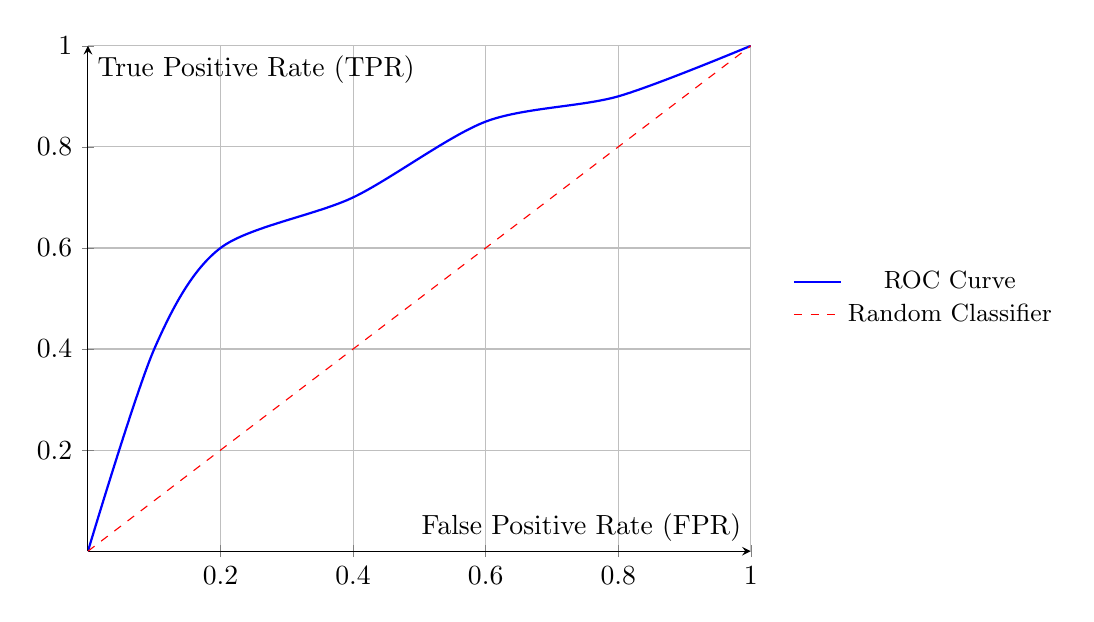
\begin{tikzpicture}
    \begin{axis}[
        width=10cm, height=8cm,
        xlabel={False Positive Rate (FPR)},
        ylabel={True Positive Rate (TPR)},
        grid=major,
        xmin=0, xmax=1,
        ymin=0, ymax=1,
        axis lines=middle,
        enlargelimits=false,
        xtick={0,0.2,0.4,0.6,0.8,1},
        ytick={0,0.2,0.4,0.6,0.8,1},
        legend style={at={(1.05,0.5)}, anchor=west, draw=none, font=\small}
      ]
      % ROC Curve
      \addplot[smooth, thick, blue] coordinates {
          (0,0) (0.1,0.4) (0.2,0.6) (0.4,0.7) (0.6,0.85) (0.8,0.9) (1,1)
        };
      \addlegendentry{ROC Curve}

      % Random classifier (diagonal line)
      \addplot[dashed, red] coordinates {(0,0) (1,1)};
      \addlegendentry{Random Classifier}
    \end{axis}
  \end{tikzpicture}
  \caption[ROC AUC Curve Example]{Example ROC Curve}
  \label{fig:roc}
  \caption*{Own tabulation based on \textcite{geron2022hands}. \ai{AI generated based on copyrighted image.}}}
\end{figure}

\begin{equation}
  \text{AUC} = \int_{0}^{1} \text{TPR}(\text{FPR}) \, d\text{FPR}
  \label{eq:auc}
\end{equation}

An ROC curve is a graphical representation that plots the true positive rate (TPR or recall) against the false positive rate (FPR) at various classification thresholds. By examining the curve, one can visualize the trade-off between the models sensitivity (its ability to correctly identify positive instances) and its specificity (its ability to correctly identify negative instances) across different decision points. The value of AUC ranges from 0 to 1. An AUC of 1 indicates a perfect classifier, while an AUC of .5 suggests a performance no better than chance level. In the context of predicting validity of data in manufacturing, a higher AUC for the network would signify that the model is better at distinguishing between valid and invalid processes, regardless of the chosen classification threshold. This is particularly valuable when the class distribution is imbalanced, as ROC and AUC provide a more robust evaluation compared to metrics like accuracy that can be skewed by the majority class \autocite{fawcett2006introduction}. Thus, ROC AUC will be used as the lead metric for assessing model quality.

Now that the basic concepts of \gls{vvuq} and the metrics used to assess model quality have been introduced, the next section will delve into the specific models employed in this work. The focus will be on the ResNet Bi-LSTM Multi-Head attention network, which is designed to automatically generate \gls{vvuq} models for \gls{sbdt}. This model unites the strengths of neural networks and attention mechanisms to handle sequential data and improve prediction accuracy.

\subsubsection*{Bidirectional LSTM Networks for Sequence-Based Anomaly Detection}

The following section describes the model types on which the automatic VBVVQ is based. The model types are introduced in a bottom-up fashion, starting with the most basic model type and building up to the more complex models.
The first model type is the Recurrent Neural Network (RNN), which is the basis for the Long Short-Term Memory (LSTM) networks. The LSTM networks are then used in a bidirectional fashion, which is the basis for the ResNet Bi-LSTM Multi-Head attention network. Because the \gls{ocel} data is sequential in nature, the RNNs are used to model the sequential data. The LSTM networks are used to overcome the limitations of the RNNs, and the bidirectional LSTM networks are used to improve the performance of the LSTM networks. The ResNet Bi-LSTM Multi-Head attention network is then introduced as a more advanced model that combines the strengths of both LSTM and attention mechanisms.\footnote{In this section, specific mathematical notation is used. Vectors, such as inputs, hidden states, cell states, outputs, and biases, are written by bold lowercase letters (e.g., \( \bm{x}, \bm{h}, \bm{c}, \bm{y}, \bm{b} \)). Matrices, primarily representing weights, are represented by uppercase letters (e.g., \( W, U \)). The symbol \( \sigma \) denotes a generic non-linear activation function, while \( \sigma_h \) and \( \sigma_y \) specifically refer to activation functions in the hidden and output layers. In \autoref{chap:case-study}, \( \sigma \) will refer to standard deviation. Commonly used specific activation functions like hyperbolic tangent and softmax are written as \( \tanh \) and \( \text{softmax} \). Element-wise multiplication is indicated by the symbol \( \odot \).}

\paragraph{\textbf{Recurrent Neural Networks (RNNs)}}
\label{sec:rnn}
Recurrent Neural Network (RNN) were the first novel networks to handle sequential data. Unlike feedforward neural networks that process each input independently, RNNs are designed to handle sequences by maintaining an internal memory, known as the hidden state, which summarizes past information \autocite{geron2022hands}. As sequential data \( \{ \bm{x}_1, \bm{x}_2, ..., \bm{x}_T \} \) is fed into the network step by step (indexed by \( t \)), the RNN processes each element \( \bm{x}_t \) while simultaneously updating its hidden state \( \bm{h}_t \). This hidden state acts as the network's memory, retaining information from previous time steps. It can be thought of as the long-term memory of the network.

The core computation within an RNN at time step \( t \) is calculating the new hidden state \( \bm{h}_t \) based on the current input \( \bm{x}_t \) and the previous hidden state \( \bm{h}_{t-1} \). This relationship is typically defined as:
\begin{equation}
  \bm{h}_t = \sigma_h (W_{xh} \bm{x}_t + W_{hh} \bm{h}_{t-1} + \bm{b}_h)
  \label{eq:rnn_hidden_state}
\end{equation}

\begin{figure}[htbp]
  \centering
  \begin{tikzpicture}[node distance=1.2cm and 1.8cm]
    % Nodes for time steps
    \node (cell_tm1) [block] {RNN};
    \node (cell_t)   [block, right=of cell_tm1] {RNN};
    \node (cell_tp1) [block, right=of cell_t] {RNN};

    % Inputs
    \node (xtm1) [below=of cell_tm1] {\(\bm{x}_{t-1}\)};
    \node (xt)   [below=of cell_t] {\(\bm{x}_t\)};
    \node (xtp1) [below=of cell_tp1] {\(\bm{x}_{t+1}\)};

    % Outputs
    \node (ytm1) [above=of cell_tm1] {\(\bm{y}_{t-1}\)};
    \node (yt)   [above=of cell_t] {\(\bm{y}_t\)};
    \node (ytp1) [above=of cell_tp1] {\(\bm{y}_{t+1}\)};

    % Hidden States (Coordinates for arrows)
    \coordinate (h_tm1_out) at (cell_tm1.east);
    \coordinate (h_t_in) at (cell_t.west);
    \coordinate (h_t_out) at (cell_t.east);
    \coordinate (h_tp1_in) at (cell_tp1.west);
    \coordinate (h_init_in) at (cell_tm1.west); % Input for h_{t-2}

    % Input Connections
    \draw [arrow] (xtm1) -- node[midway, right, font=\footnotesize]{$W_{xh}$} (cell_tm1);
    \draw [arrow] (xt)   -- node[midway, right, font=\footnotesize]{$W_{xh}$} (cell_t);
    \draw [arrow] (xtp1) -- node[midway, right, font=\footnotesize]{$W_{xh}$} (cell_tp1);

    % Output Connections
    \draw [arrow] (cell_tm1) -- node[midway, right, font=\footnotesize]{$W_{hy}$} (ytm1);
    \draw [arrow] (cell_t)   -- node[midway, right, font=\footnotesize]{$W_{hy}$} (yt);
    \draw [arrow] (cell_tp1) -- node[midway, right, font=\footnotesize]{$W_{hy}$} (ytp1);

    % Hidden State Connections (Recurrence)
    \draw [arrow] (h_tm1_out) -- node[midway, above]{$\bm{h}_{t-1}$} node[midway, below, font=\footnotesize]{$W_{hh}$} (h_t_in);
    \draw [arrow] (h_t_out)   -- node[midway, above]{$\bm{h}_{t}$} node[midway, below, font=\footnotesize]{$W_{hh}$} (h_tp1_in);

    % Indicate initial / further connections
    \node (dots_left_h) [left=0.8cm of h_init_in] {\(\dots\)};
    \draw [arrow] (dots_left_h) -- node[midway, above]{$\bm{h}_{t-2}$} node[midway, below, font=\footnotesize]{$W_{hh}$} (h_init_in);
    \node (dots_right_h) [right=0.8cm of cell_tp1] {\(\dots\)};
    \draw [arrow] (cell_tp1) -- (dots_right_h); % Arrow towards further steps

    % Ellipses for sequences
    \node (dots_left_x) [left=0.8cm of xtm1] {\(\dots\)};
    \draw [arrow] (dots_left_x) -- (xtm1);
    \node (dots_right_x) [right=0.8cm of xtp1] {\(\dots\)};
    \draw [arrow] (xtp1) -- (dots_right_x);

    \node (dots_left_y) [left=0.8cm of ytm1] {\(\dots\)};
    \draw [arrow] (ytm1) -- (dots_left_y);
    \node (dots_right_y) [right=0.8cm of ytp1] {\(\dots\)};
    \draw [arrow] (ytp1) -- (dots_right_y);

  \end{tikzpicture}
  \caption[RNN Unfolded]{Unfolded architecture of a Recurrent Neural Network over time, illustrating the computation of the hidden state \(\bm{h}_t\) according to \autoref{eq:rnn_hidden_state}.}
  \label{fig:rnn_unfolded}
  \caption*{Illustration based on \textcite{geron2022hands}. \ai{AI generated based on copyrighted image.}}
\end{figure}

where \( W_{xh} \) is the weight matrix connecting the input to the hidden layer, \( W_{hh} \) is the weight matrix for the recurrent connection from the previous hidden state to the current hidden state, \( \bm{b}_h \) is the bias vector for the hidden layer, and \( \sigma_h \) is a non-linear activation function, commonly the hyperbolic tangent (\(\tanh\)) or ReLU. The initial hidden state \( \bm{h}_0 \) is typically initialized to zeros or learned.

The output \( \bm{y}_t \) at time step \( t \) can then be computed from the hidden state:
\begin{equation}
  \bm{y}_t = \sigma_y (W_{hy} \bm{h}_t + \bm{b}_y)
  \label{eq:rnn_output}
\end{equation}
Here, \( W_{hy} \) is the weight matrix from the hidden layer to the output layer, \( \bm{b}_y \) is the output bias vector, and \( \sigma_y \) is an activation function suitable for the task, for example softmax for classification tasks.

One characteristic of RNNs is \textit{parameter sharing}: The weight matrices (\( W_{xh}, W_{hh}, W_{hy} \)) and biases (\( \bm{b}_h, \bm{b}_y \)) are the same across all time steps \( t = 1, ..., T \). This allows the model to generalize learned patterns regardless of their position in the sequence and reduces the number of parameters to learn. This process is often understood by thinking of the network as being `unfolded' over time, creating a deep feedforward-like structure where each layer corresponds to a time step but utilizes shared weights \autocite{medsker2001recurrent}.

In contrast to their conceptual innovation, standard RNNs face challenges when learning dependencies over long sequences. During training using Backpropagation Through Time (BPTT), gradients are propagated backward through the unfolded network representation. The repeated multiplication involving the recurrent weight matrix \( W_{hh} \) (specifically, its Jacobian matrix containing the first derivatives) can cause gradients to either shrink exponentially towards zero (vanishing gradients) or grow uncontrollably (exploding gradients) \autocite{hochreiter1998vanishing}. Vanishing gradients hinder the models ability to capture long-range dependencies, as updates to weights connecting distant past inputs become negligible. Exploding gradients can lead to numerical instability during training \autocite{philipp2017exploding}.

\paragraph{\textbf{Long Short-Term Memory Networks (LSTMs)}}
\label{sec:lstm}

To address the vanishing gradient problem and learn long-range dependencies, Long Short-Term Memory Networks (LSTMs) were introduced \autocite{hochreiter1997long}. LSTMs have a more advanced internal structure within each recurrent unit, often called an LSTM cell.

The key innovation of the LSTM cell is the introduction of a \textit{cell state}, \( \bm{c}_t \), which acts as an information conduit, allowing information to flow through time with minimal modification. The long-term preservation is a key distinction from the RNN, where the hidden state gets overwritten. The flow of information into, out of, and within the cell state is regulated by three specialized gating mechanisms: the forget gate, the input gate, and the output gate. These gates use sigmoid activation functions (\(\sigma\)), which output values between 0 and 1, representing the proportion of information allowed to pass.

\begin{figure}[htbp]
  \centering
  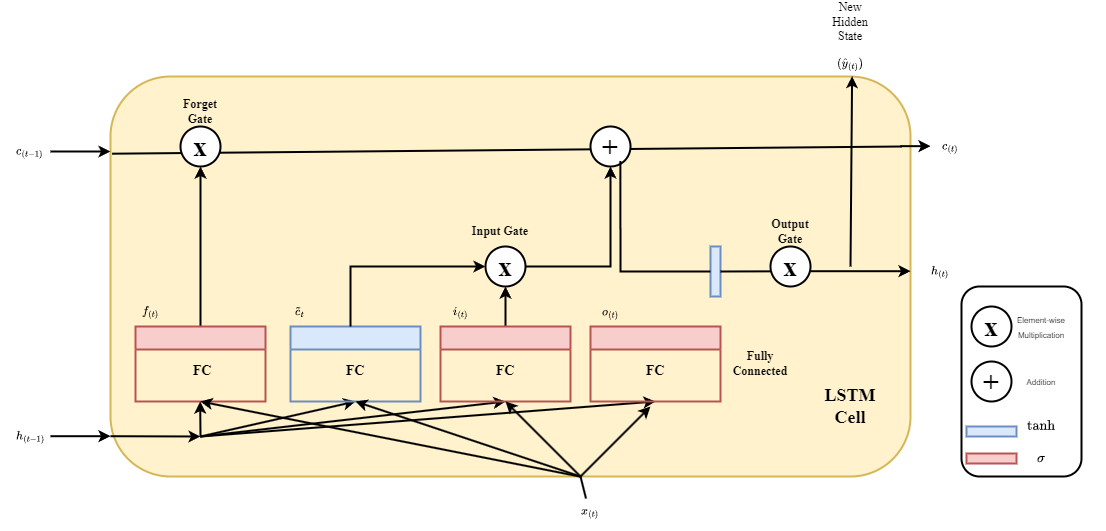
\includegraphics[width=0.8\textwidth]{figures/lstmcell.png}
  \caption[LSTM Cell]{Visual representation of the LSTM cell computations detailed in Equations \ref{eq:lstm-forget-gate} to \ref{eq:lstm-hidden-state}. The diagram shows how inputs $\bm{x}_t$ and $\bm{h}_{t-1}$ interact with the forget gate ($\bm{f}_t$), input gate ($\bm{i}_t$), candidate state ($\bm{\tilde{c}}_t$), and output gate ($\bm{o}_t$) to update the cell state from $\bm{c}_{t-1}$ to $\bm{c}_t$ and compute the hidden state $\bm{h}_t$.}
  \caption*{Source: Own illustration based on \autocite{geron2022hands}.}
  \label{fig:lstm_cell}
\end{figure}
At each time step \( t \), given the input \( \bm{x}_t \), the previous hidden state \( \bm{h}_{t-1} \), and the previous cell state \( \bm{c}_{t-1} \), the LSTM cell does the following computations:

\begin{enumerate}
  \item \textbf{Forget Gate (\( \bm{f}_t \)):} Decides which information to forget from the previous cell state \( \bm{c}_{t-1} \).
        \begin{equation}
          \bm{f}_t = \sigma(W_f \bm{x}_t + U_f \bm{h}_{t-1} + \bm{b}_f)
          \label{eq:lstm-forget-gate}
        \end{equation}

  \item \textbf{Input Gate (\( \bm{i}_t \)):} Determines which new information from the input and previous hidden state should be added in the cell state. This involves two parts:
        \begin{itemize}
          \item The input gate layer decides which values to update:
                \begin{equation}
                  \bm{i}_t = \sigma(W_i \bm{x}_t + U_i \bm{h}_{t-1} + \bm{b}_i)
                  \label{eq:lstm-input-gate}
                \end{equation}
          \item A candidate cell state \( \bm{\tilde{c}}_t \) is created with potential new values, typically using a \( \tanh \) activation:
                \begin{equation}
                  \bm{\tilde{c}}_t = \tanh(W_c \bm{x}_t + U_c \bm{h}_{t-1} + \bm{b}_c)
                  \label{eq:lstm-candidate-cell}
                \end{equation}
        \end{itemize}

  \item \textbf{Cell State Update (\( \bm{c}_t \)):} The old cell state \( \bm{c}_{t-1} \) is updated to the new cell state \( \bm{c}_t \). This involves element-wise multiplication (\(\odot\)) to forget parts of the old state (via \( \bm{f}_t \)) and add parts of the new candidate state (via \( \bm{i}_t \)).
        \begin{equation}
          \bm{c}_t = \bm{f}_t \odot \bm{c}_{t-1} + \bm{i}_t \odot \bm{\tilde{c}}_t
          \label{eq:lstm-cell-update}
        \end{equation}

  \item \textbf{Output Gate (\( \bm{o}_t \)):} Determines what part of the (filtered) cell state \( \bm{c}_t \) should be outputted as the new hidden state \( \bm{h}_t \).
        \begin{equation}
          \bm{o}_t = \sigma(W_o \bm{x}_t + U_o \bm{h}_{t-1} + \bm{b}_o)
          \label{eq:lstm-output-gate}
        \end{equation}
        \begin{equation}
          \bm{h}_t = \bm{o}_t \odot \tanh(\bm{c}_t)
          \label{eq:lstm-hidden-state}
        \end{equation}
\end{enumerate}

In these equations, \( W_*, U_* \) represent the weight matrices for connections from the input and the previous hidden state, and \( \bm{b}_* \) are the bias vectors.

The gating mechanisms allow LSTMs to selectively remember or forget information over long durations. The cell state's update mechanism, involving addition and element-wise multiplication controlled by gates often close to 1 (especially the forget gate), supports a more stable gradient flow compared to the repeated matrix multiplications in simple RNNs. This characteristic, sometimes associated with the Constant Error Carousel (CEC) concept \autocite{hochreiter1997long}, effectively mitigates the vanishing gradient problem. LSTMs have become a standard tool for various sequence modelling tasks, including time series prediction and machine sequences \autocite{al2024rnn}.


\paragraph{\textbf{Bidirectional LSTMs (Bi-LSTMs)}}
\label{sec:bilstm}

\begin{figure}[htbp]
  \centering
  \begin{tikzpicture}[node distance=0.6cm and 1.3cm]
    % Input Sequence
    \node (x1) {\(\dots\)};
    \node (x2) [right=of x1] {\(\bm{x}_{t-1}\)};
    \node (x3) [right=of x2] {\(\bm{x}_t\)};
    \node (x4) [right=of x3] {\(\bm{x}_{t+1}\)};
    \node (x5) [right=of x4] {\(\dots\)};
    \node[below=1.5em of x3, text width=6cm, align=center] {Input Sequence};

    % Forward LSTM Layer
    \node (f1) [block, fill=blue!20, above=1.2cm of x1] {\(\rightarrow\)};
    \node (f2) [block, fill=blue!20, above=1.2cm of x2] {\(\rightarrow\)};
    \node (f3) [block, fill=blue!20, above=1.2cm of x3] {\(\rightarrow\)};
    \node (f4) [block, fill=blue!20, above=1.2cm of x4] {\(\rightarrow\)};
    \node (f5) [block, fill=blue!20, above=1.2cm of x5] {\(\rightarrow\)};
    \node[left=0.5em of f1, text width=2cm, align=right] {Forward LSTM};

    % Backward LSTM Layer
    \node (b1) [block, fill=orange!20, above=0.8cm of f1] {\(\leftarrow\)};
    \node (b2) [block, fill=orange!20, above=0.8cm of f2] {\(\leftarrow\)};
    \node (b3) [block, fill=orange!20, above=0.8cm of f3] {\(\leftarrow\)};
    \node (b4) [block, fill=orange!20, above=0.8cm of f4] {\(\leftarrow\)};
    \node (b5) [block, fill=orange!20, above=0.8cm of f5] {\(\leftarrow\)};
    \node[left=0.5em of b1, text width=2cm, align=right] {Backward LSTM};

    % Combined Output Layer (representing concatenation)
    \coordinate (c1) at ($(f1)!0.5!(b1) + (0,1.5cm)$); % Position above the two layers
    \coordinate (c2) at ($(f2)!0.5!(b2) + (0,1.5cm)$);
    \coordinate (c3) at ($(f3)!0.5!(b3) + (0,1.5cm)$);
    \coordinate (c4) at ($(f4)!0.5!(b4) + (0,1.5cm)$);
    \coordinate (c5) at ($(f5)!0.5!(b5) + (0,1.5cm)$);

    % Output Nodes/Labels
    \node (o1) [above=0.1cm of c1] {\(\dots\)};
    \node (o2) [above=0.1cm of c2] {\(\bm{h}_{t-1}\)};
    \node (o3) [above=0.1cm of c3] {\(\bm{h}_t\)};
    \node (o4) [above=0.1cm of c4] {\(\bm{h}_{t+1}\)};
    \node (o5) [above=0.1cm of c5] {\(\dots\)};
    \node[above=1.5em of o3, text width=6cm, align=center] {Combined Output Sequence};


    % Input Arrows to both LSTMs
    \draw[arrow] (x1) |- (f1.south); \draw[arrow] (x1) |- (b1.south);
    \draw[arrow] (x2) -- (f2.south); \draw[arrow] (x2) -- (b2.south);
    \draw[arrow] (x3) -- (f3.south); \draw[arrow] (x3) -- (b3.south);
    \draw[arrow] (x4) -- (f4.south); \draw[arrow] (x4) -- (b4.south);
    \draw[arrow] (x5) |- (f5.south); \draw[arrow] (x5) |- (b5.south);

    % LSTM Layer Connections (Forward)
    \draw[arrow] (f1) -- node[midway, above, font=\tiny]{\(\vec{\bm{h}}_{t-2}\)} (f2);
    \draw[arrow] (f2) -- node[midway, above, font=\tiny]{\(\vec{\bm{h}}_{t-1}\)} (f3);
    \draw[arrow] (f3) -- node[midway, above, font=\tiny]{\(\vec{\bm{h}}_{t}\)} (f4);
    \draw[arrow] (f4) -- node[midway, above, font=\tiny]{\(\vec{\bm{h}}_{t+1}\)} (f5);

    % LSTM Layer Connections (Backward)
    \draw[arrow] (b5) -- node[midway, below, font=\tiny]{\(\cev{\bm{h}}_{t+2}\)} (b4);
    \draw[arrow] (b4) -- node[midway, below, font=\tiny]{\(\cev{\bm{h}}_{t+1}\)} (b3);
    \draw[arrow] (b3) -- node[midway, below, font=\tiny]{\(\cev{\bm{h}}_{t}\)} (b2);
    \draw[arrow] (b2) -- node[midway, below, font=\tiny]{\(\cev{\bm{h}}_{t-1}\)} (b1);

    % Output Arrows (Combining)
    \draw[arrow] (f1.north) -- (c1); \draw[arrow] (b1.north) -- (c1);
    \draw[arrow] (f2.north) -- node[midway, left, font=\tiny]{\(\vec{\bm{h}}_{t-1}\)} (c2);
    \draw[arrow] (b2.north) -- node[midway, right, font=\tiny]{\(\cev{\bm{h}}_{t-1}\)} (c2);
    \draw[arrow] (f3.north) -- node[midway, left, font=\tiny]{\(\vec{\bm{h}}_{t}\)} (c3);
    \draw[arrow] (b3.north) -- node[midway, right, font=\tiny]{\(\cev{\bm{h}}_{t}\)} (c3);
    \draw[arrow] (f4.north) -- node[midway, left, font=\tiny]{\(\vec{\bm{h}}_{t+1}\)} (c4);
    \draw[arrow] (b4.north) -- node[midway, right, font=\tiny]{\(\cev{\bm{h}}_{t+1}\)} (c4);
    \draw[arrow] (f5.north) -- (c5); \draw[arrow] (b5.north) -- (c5);

    % Arrows to final output nodes
    \draw[arrow] (c1) -- (o1);
    \draw[arrow] (c2) -- (o2);
    \draw[arrow] (c3) -- (o3);
    \draw[arrow] (c4) -- (o4);
    \draw[arrow] (c5) -- (o5);

    % Annotation for combination
    \node[draw, ellipse, dashed, fit=(f3)(b3), inner 09 = 0.3cm, label={[yshift=-1.2cm]center:Combine}] {};
  \end{tikzpicture}
  \caption[Bi-LSTM Architecture]{Architecture of a Bidirectional LSTM (Bi-LSTM), processing the input sequence (\(\bm{x}_t\)) both forwards (generating \(\vec{\bm{h}}_t\)) and backwards (generating \(\cev{\bm{h}}_t\)). The final hidden states \(\bm{h}_t\) are produced by combining information from both directions (via concatenation according to Equation \autoref{eq:bilstm_concat}).}
  \label{fig:bilstm_arch}
  \caption*{\ai{AI generated based on copyrighted image.}}
\end{figure}

While standard LSTMs process sequences chronologically, capturing dependencies on past inputs, many tasks benefit from considering context from both past and future elements. For example, understanding why a specific machine task is performed requires knowledge about the task performed afterwards. Bidirectional LSTMs (Bi-LSTMs) address this by processing the input sequence in both forward and backward directions \autocite{schuster1997bidirectional}.

A Bi-LSTM consists of two separate LSTM layers:

\begin{enumerate}
  \item A \textbf{forward LSTM} processes the input sequence \( \{\bm{x}_1, ..., \bm{x}_T\} \) from \( t=1 \) to \( T \), producing a sequence of forward hidden states \( \{\vec{\bm{h}}_1, ..., \vec{\bm{h}}_T\} \). The computation for \( \vec{\bm{h}}_t \) follows the standard LSTM equations \autoref{eq:lstm-forget-gate} through \autoref{eq:lstm-hidden-state}.
  \item A \textbf{backward LSTM} processes the input sequence in reverse order, from \( t=T \) down to \( 1 \), producing a sequence of backward hidden states \( \{\cev{\bm{h}}_1, ..., \cev{\bm{h}}_T\} \). The computation for \( \cev{\bm{h}}_t \) uses a separate set of LSTM parameters and processes the sequence \( \{\bm{x}_T, ..., \bm{x}_1\} \).
\end{enumerate}

At each time step \( t \), the final hidden state representation \( \bm{h}_t \) combines the information from both directions. A common method is concatenation:
\begin{equation}
  \bm{h}_t = [\vec{\bm{h}}_t ; \cev{\bm{h}}_t]
  \label{eq:bilstm_concat}
\end{equation}
where \( [;] \) denotes vector concatenation. Other combination methods like summation or averaging are also possible. This combined state \( \bm{h}_t \) contains information about the input \( \bm{x}_t \) informed by both its preceding and succeeding context within the sequence.

Bi-LSTMs have proven effective in tasks requiring contextual understanding, such as Named Entity Recognition or sentiment analysis \autocite{al2024rnn}. They have not been applied widely in the manufacturing domain. Unfortunately, they are computationally more expensive than unidirectional LSTMs due to the doubled network structure.

\paragraph{\textbf{Residual Networks (ResNets)}}
\label{sec:resnet}

As neural networks became deeper to model more complex functions, researchers encountered the \textit{degradation problem}: simply stacking more layers could lead to higher training error, even though a deeper network should theoretically be able to represent the functions learned by a shallower one \autocite{he2016deep}. This issue, different from overfitting, showed difficulties in optimizing very deep networks. Residual Networks (ResNets) were introduced to overcome this challenge. The core idea is to reframe the learning process by having layers learn a \textit{residual function} with respect to their input, rather than learning the desired underlying mapping directly. This is achieved using \textit{residual blocks} containing skip connections (or shortcut connections).

Such a block of layers aiming to learn a mapping is denoted \( \mathcal{H}(\bm{x}) \). A residual block instead learns a residual function \( \mathcal{F}(\bm{x}) = \mathcal{H}(\bm{x}) - \bm{x} \). The output \( \bm{y} \) of the residual block is then computed as:
\begin{equation}
  \bm{y} = \mathcal{F}(\bm{x}, \{W_i\}) + \bm{x}
  \label{eq:resnet_block}
\end{equation}
Here, \( \bm{x} \) is the input to the block, \( \mathcal{F}(\bm{x}, \{W_i\}) \) is the function learned by the stacked layers within the block (described by weights \( \{W_i\} \)), and the \( +\bm{x} \) term is an identity skip connection. This formulation makes it easier for the network to learn an identity mapping by driving the weights in \( \mathcal{F} \) towards zero.

These skip connections provide alternative pathways for gradient propagation during backpropagation. Gradients can flow directly through the identity connections, overjumping the layers in \( \mathcal{F} \). This avoids the vanishing gradient problem in very deep networks, allowing for the successful training of models with hundreds or even thousands of layers \autocite{he2016deep}. While originally developed for computer vision, the principle of residual connections can be applied to other architectures, including sequential models. Using ResNet-like connections within or around (Bi-)LSTM layers can stabilize training and allow for deeper sequential architectures, enabling the capture of more  temporal patterns without suffering from degradation.

\paragraph{\textbf{Multi-head Attention Mechanism}}
\label{sec:attention}
In sequence modelling, particularly with long sequences, not all parts of the input are equally relevant for making a prediction at a given time step. Attention mechanisms allow a model to dynamically focus on the most important parts of the input sequence \autocite{chorowski2014end}. A core idea is \textit{self-attention}, where the mechanism relates different positions of a single sequence to compute its representation \autocite{vaswani2017attention}.

Self-attention works on input vectors, typically representing tokens or time steps in a sequence. For each input vector, three representations are learned through linear transformations: a query (\( \bm{q} \)), a key (\( \bm{k} \)), and a value (\( \bm{v} \)). The attention mechanism computes the output as a weighted sum of the values, where the weight assigned to each value is determined by the compatibility (often measured by dot product) between its corresponding key and the query.

The most common form is \textit{Scaled Dot-Product Attention}, calculated for a set of queries \( Q \), keys \( K \), and values \( V \) (where \( Q, K, V \) are matrices stacking the \( \bm{q}, \bm{k}, \bm{v} \) vectors):
\begin{equation}
  \text{Attention}(Q, K, V) = \text{softmax}\left(\frac{QK^T}{\sqrt{d_k}}\right) V
  \label{eq:scaled_dot_product_attention}
\end{equation}
Here, \( QK^T \) computes the dot products between all query-key pairs. The result is scaled by \( \sqrt{d_k} \), where \( d_k \) is the dimension of the keys, to prevent the dot products from becoming too large and pushing the softmax function into regions with very small gradients. The softmax function normalizes these scores into attention weights, which sum to 1. Finally, these weights are multiplied by the Value matrix \( V \) to produce the output, highlighting the values corresponding to the most relevant keys for each query.

\textit{Multi-Head Attention} enhances this mechanism by performing the attention calculation multiple times in parallel, each with different, learned linear projections of the original \( Q, K, V \). This allows the model to jointly attend to information from different representation subspaces at different positions \autocite{vaswani2017attention}.

Let the number of heads be \( h \). For each head \( i \in \{1, ..., h\} \), the input \( Q, K, V \) are projected using learned weight matrices \( W^Q_i, W^K_i, W^V_i \):
\begin{equation}
  \text{head}_i = \text{Attention}(Q W^Q_i, K W^K_i, V W^V_i)
  \label{eq:attention_head_i}
\end{equation}
The outputs of all heads are then concatenated and projected one final time using another learned weight matrix \( W^O \):
\begin{equation}
  \text{MultiHead}(Q, K, V) = \text{Concat}(\text{head}_1, ..., \text{head}_h) W^O
  \label{eq:multihead_attention}
\end{equation}

This multi-head structure allows each head to potentially focus on different types of relationships, leading to a richer representation. Multi-head attention is a cornerstone of the transformer architecture \autocite{vaswani2017attention} and is increasingly combined with other models like LSTMs.

\paragraph{\textbf{The Integrated Architecture for Anomaly Detection}}
\label{sec:integrated_architecture}

The theoretical components described above can be integrated. For the challenge of anomaly detection in sequential manufacturing process data within the context of \gls{sbdt}, an architecture combining these elements offers significant advantages. The proposed model utilizes Bi-LSTM layers as the core sequence processing units to capture the temporal dynamics inherent in manufacturing operations, using their ability to model long-range dependencies as described in \autoref{sec:lstm} and \autoref{sec:bilstm}. To potentially enable deeper Bi-LSTM stacks and stabilize training, residual connections, inspired by ResNet principles ( \autoref{sec:resnet}), can be incorporated within or between these layers. Following the Bi-LSTM layers, a multi-head attention mechanism (\autoref{sec:attention}) is applied to the sequence of hidden states generated by the Bi-LSTMs. This allows the model to adaptively weigh the importance of different time steps or features in the sequence when making a final prediction. By focusing on the most salient parts of the process history, the attention mechanism can enhance the models ability to distinguish between normal and anomalous patterns. The multi-head approach enables simultaneous focus on diverse aspects potentially indicative of anomalies. The final output of the attention layer is passed through further feedforward layers to produce the anomaly classification (a probability score indicating deviation from normal behaviour). This integrated architecture aims to use the strengths of each component: Temporal modelling from Bi-LSTMs, improved trainability from residual connections, and context-aware focusing from multi-head attention.

The architecture directly relates to the \gls{vvuq} of \gls{sbdt}s. Accurate anomaly classification serves as a form of validation for the \gls{dt}s representation of normal process behaviour. Analysing the attention weights (derived from \autoref{eq:scaled_dot_product_attention}) can provide insights into which process steps or features the model considers most indicative of anomalies, helping in the verification and interpretation of both the model and the manufacturing process itself. UQ is then performed by conducting statistical significance testing. The next chapter will describe modern \gls{vvuq} techniques within the \gls{sbdt} context.


\subsection{Modern VVUQ in the Context of SBDT}
\label{sec:vvuq-dt}
ML-based \gls{vvuq} approaches heavily rely on data. In the preceding sections, the thesis introduced several interfaces which may serve as suitable data sources. \gls{pm}/\gls{oced} may provide event logs for \gls{vvuq} approaches. \gls{ml} approaches can ingest those. \gls{ppc} systems may provide additional data to enrich the event log. This section will shed light on a systematic literature review (SLR) on V\&V in the context of \gls{dt}s. After summarizing the main findings, several V\&V approaches with increasing sophistication are presented. The section closes with a discussion of the most promising approaches.

\Textcite{Bitencourt2023} conducted a SLR on V\&V in the context of \gls{dt}, a relatively new field. They did not consider uncertainty quantification in their SLR. As \textcite{hua2022validation} note, there are no structured and established frameworks for validating \gls{dt}s. This statement holds for all sectors where \gls{dt}s are applied. The SLR analysed 269 papers. They applied the 4R framework by \textcite{Osho2022jmsy} to describe the capabilities of the analysed twin frameworks. The 4R framework consists of the four dimensions \textit{Representation}, \textit{Replication}, \textit{Reality} and \textit{Relational}. The SLR found that most frameworks ($49\%$) rather developed a \gls{dm} or \gls{ds}. Another $26\%$ of \gls{dt} were only able to \textit{represent} the physical entity. Highly sophisticated \gls{dt} were the exception, not the rule. Considering this trend, V\&V may not be a topic researchers are interested in at first sight. \Textcite{Bitencourt2023} identified a trend throughout the years of increasing modelling capabilities of the considered \gls{dt}. Up to the year 2023, the trend is still increasing. They identify more data sources as the main driver for this trend. From the 269 papers, $47\%$ have been applied in the manufacturing domain. Of all classified \gls{dt}, one key insight is that most authors performed at least one form of V\&V.

\begin{figure}[htbp]
  \centering
  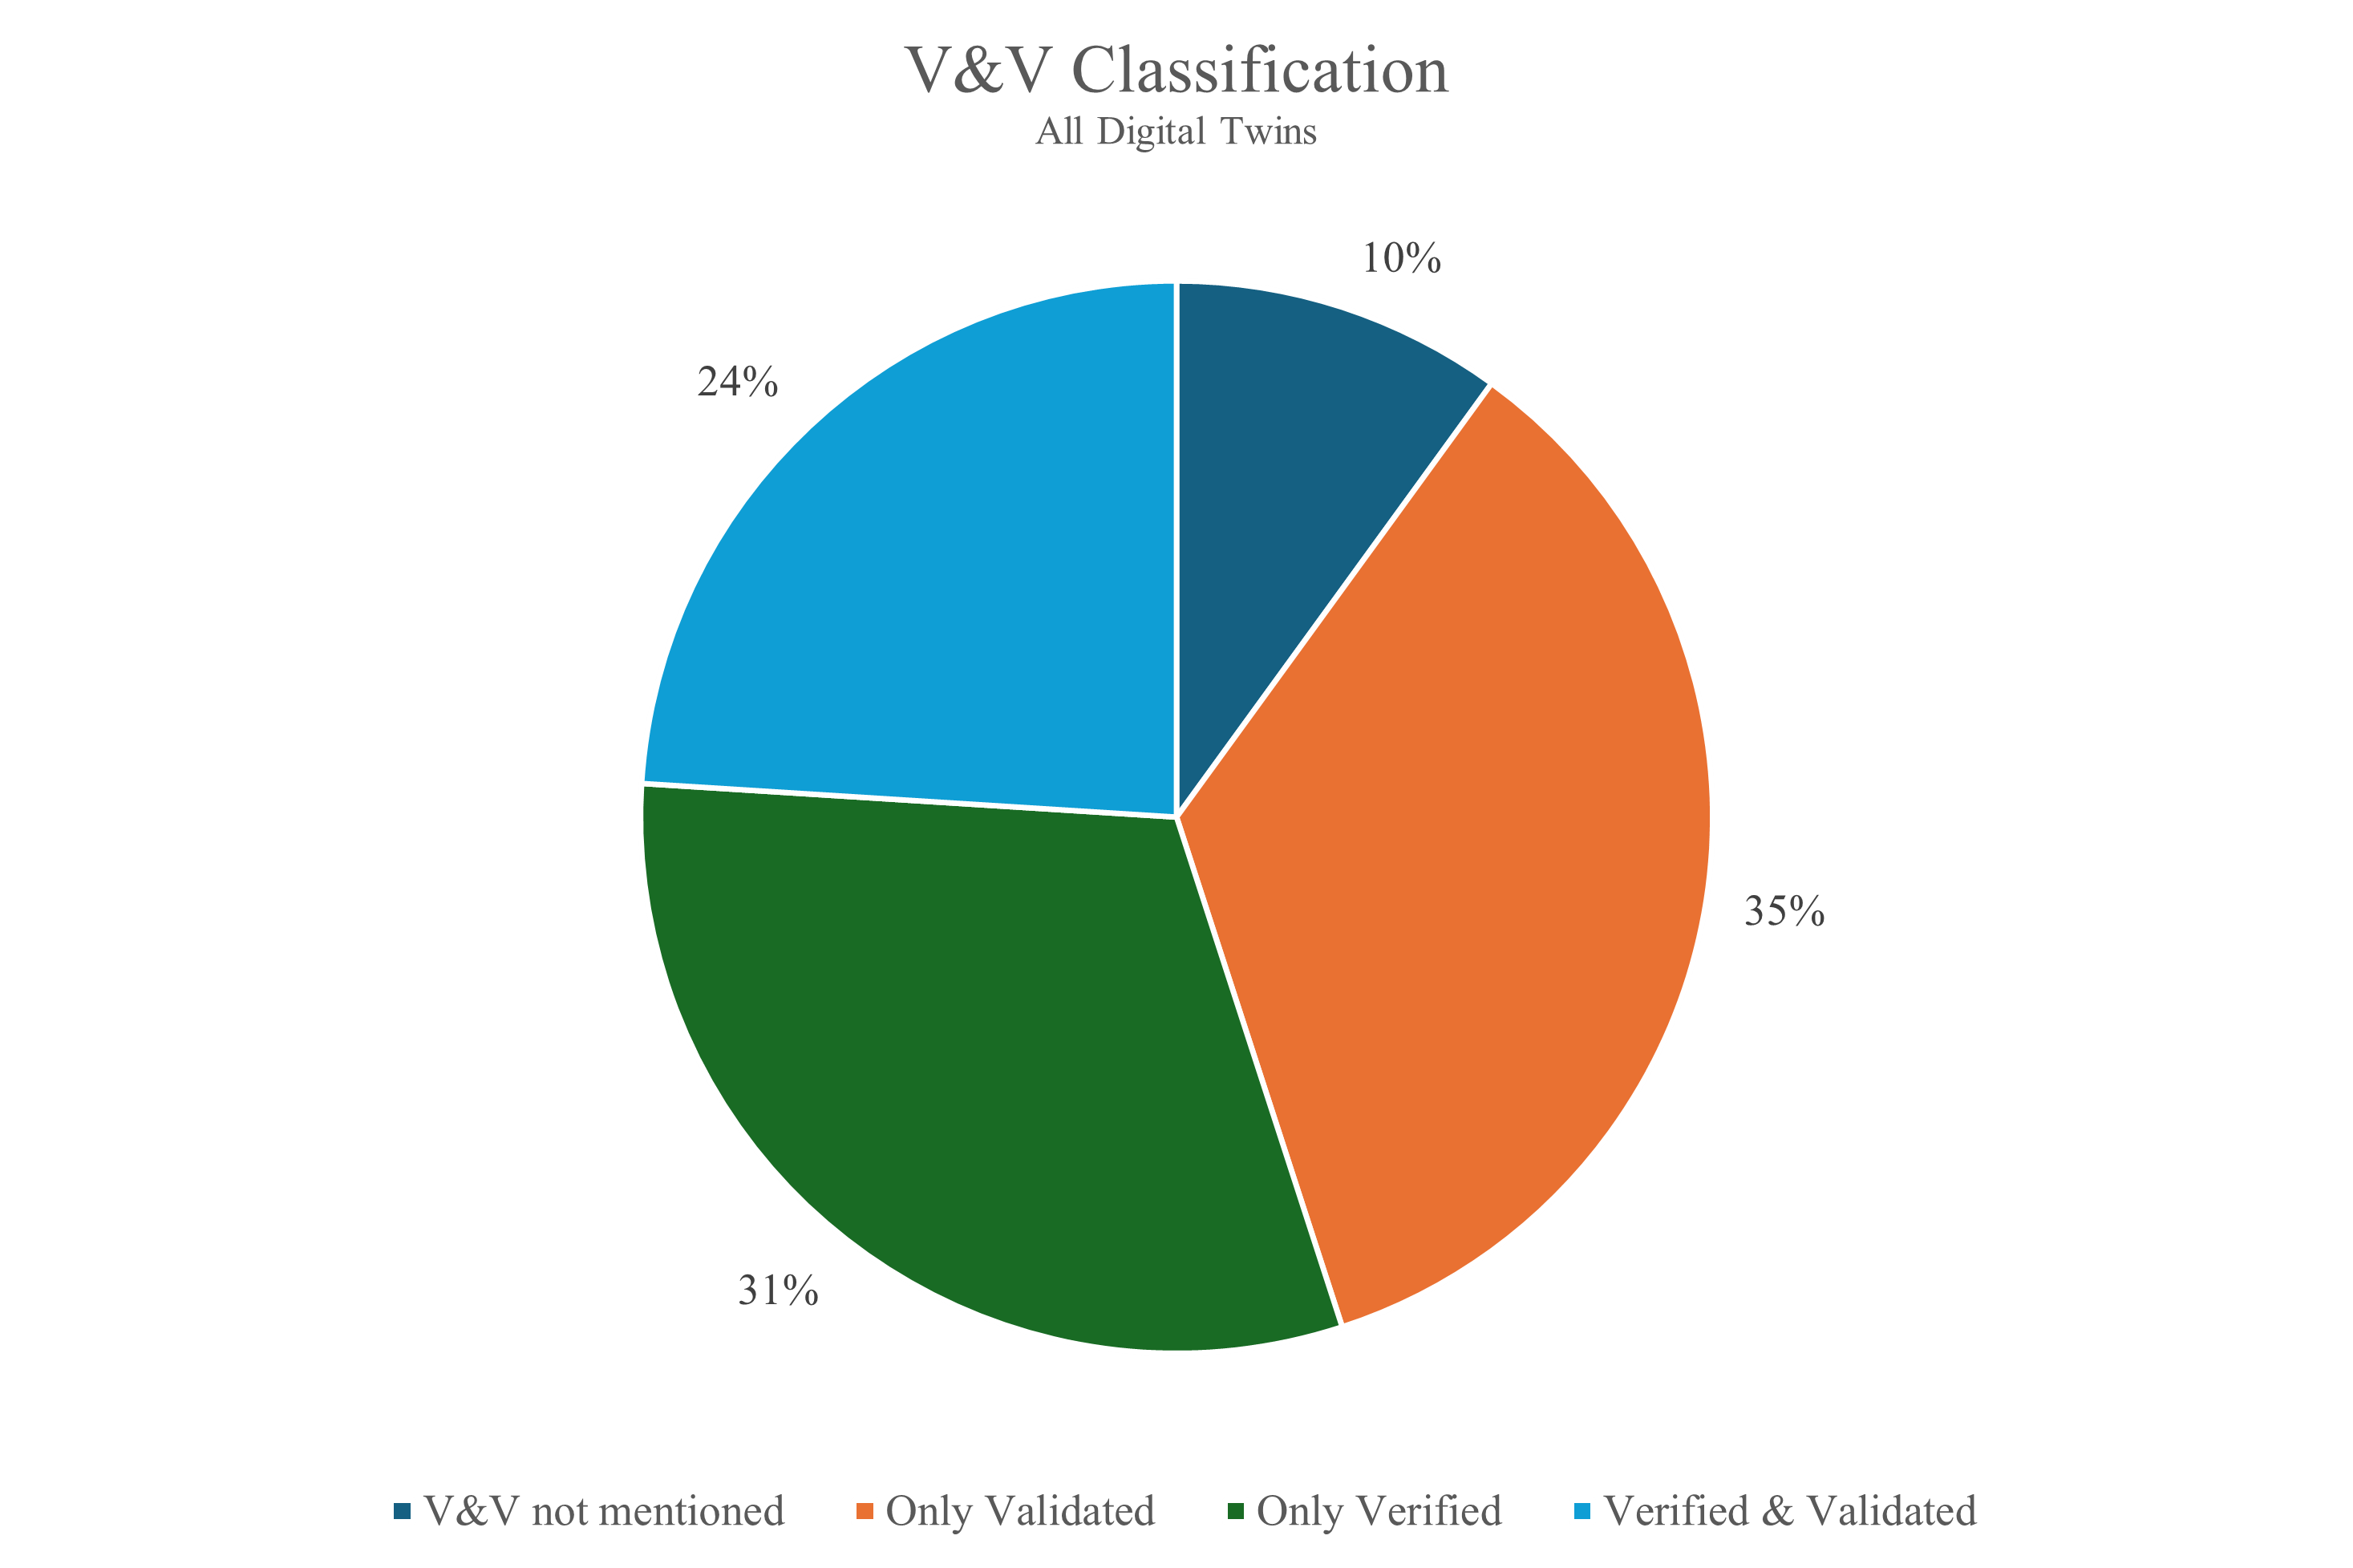
\includegraphics[width=0.8\textwidth]{figures/vvbitencourt.png}
  \caption[Donut Chart V\&V]{Donut chart showing the distribution of V\&V methods in the context of \gls{dt}.}
  \label{fig:vvbitencourt}
  \caption*{Own illustration based on \textcite{Bitencourt2023}.}
\end{figure}

\gls{dt}s ranking in the \textit{reality} category where most often verified and validated. The authors deduce that because of the increasing complexity of the model, V\&V may become a stressing topic. \Textcite{Nie2023rcim} propose a multi-agent and cloud-edge orchestration framework leveraging \gls{dt} and IIoT to optimize distributed manufacturing resources. Their framework integrates a Convolutional Neural Network (CNN) with a bidirectional Long Short Term Memory (LSTM) module to perform scheduling and self-adaptive strategies for intelligent, real-time production control. They compare their network with an earlier adopted algorithm and its result to perform V\&V. Quantifying the validity, they use Mean Squared Error (MSE) and Mean Absolute Error (MAE), see \autoref{sec:metrics-theory}.
\Textcite{Lv2023rcim} defined target scenarios and boundaries to verify their \gls{dt} for fault diagnosis of a drilling platform. They defined intervals for the metrics to be valid. Validation was performed by conducting a case study. Latter can be termed qualitative validation because the factual similarity of the case study against the \gls{dt} has been assessed. Regarding their verification approach, they go one step further than \textcite{Nie2023rcim} by defining control intervals. This is somewhat automatic verification, but still requires human intervention when the values leave the defined intervals. \Textcite{Chen2023,Mykoniatis2021jim} both performed visual inspection to verify their \gls{dt}. Both used cameras or other visual inspection tools to compare the \gls{dt} results with reality. \Textcite{Chen2023} used thermal cameras to conduct temperature scans and compared the results with temperature prediction of the twin. \Textcite{Mykoniatis2021jim} used video recordings to validate their twin behaviour, but consulted KPIs to further validate their twin. Both approaches use aids for measurements and visual inspection. The measurements still have to be conducted and compared manually. Some authors performed statistical V\&V, although the measurements were not automated. \Textcite{Wang2023asoc} compared historical data with the twin data and calculated the mean absolute percentage error of both datasets, \autoref{sec:metrics-theory}. For validation they relied on conducting a case study, thus not fully automating V\&V. \Textcite{Min2019ijinfomgt} performed verification using \gls{ppc} KPIs, automating the V\&V process even further. Their validation included using a validation set and measuring a set of metrics including error of fit and accuracy. This approach can be considered the first step towards a fully automated \gls{vvuq} process. \Textcite{Bitencourt2023} conclude that the majority of the analysed papers performed V\&V manually, with only a few authors automating the process. They also note that most authors did not consider uncertainty quantification in their work. And indeed, most work was performed in only conducting verification ($31\%$) where case studies were the method of choice \autocite{Eunike2022,jia2023from,kumbhar2023digital,Leng2020rcim,Leng2022aei}}. Case studies were also often applied where only validation took place ($35\%$) \autocite{Alam2023,Dobaj2022,kherbache2022digital,Latsou2023,Leng2021jclepro,Negri2019promfg}. The SLR shows that V\&V is a topic of interest in the context of \gls{dt}, but most authors still rely on manual methods. The trend towards more sophisticated \gls{dt}s and the increasing complexity of models will likely drive further research in this area. The SLR also highlights the need for more automated and standardized V\&V processes, especially in the context of uncertainty quantification. Very few authors performed fully automated \gls{vvuq} for \gls{dt}. The ones who did will now be discussed in more detail.


\subsubsection*{K-Nearest Neighbours (KNN) for Digital Twin Accreditation in Manufacturing}
\label{sec:knn}
The k-Nearest Neighbours (KNN) algorithm, a lazy learning approach grounded in measuring feature similarity, can be used for the accreditation of manufacturing \gls{dt}s \autocite{dos2024simulation}. KNN classifies new data points by identifying the majority class among the $K$ nearest neighbours in the training dataset. The determination of ``being close' relies on various distance metrics. Most commonly, the Euclidean distance (see \autoref{eq:euclidean_distance} is used. Selecting an appropriate value for $K$ is crucial for balancing the models bias and variance. A small $K$ can lead to overfitting, while a large $K$ may provide no insights at all. It is not an eager learner like DTrees or NN because it does not learn a model from the training data. Instead, it stores the training data and makes predictions based on the stored data. This characteristic makes KNN particularly suitable for scenarios where the underlying distribution of the data is unknown or complex. The algorithm's simplicity and interpretability make it a popular choice for various classification tasks, including those in manufacturing contexts.

\begin{figure}[htbp]
  \centering
  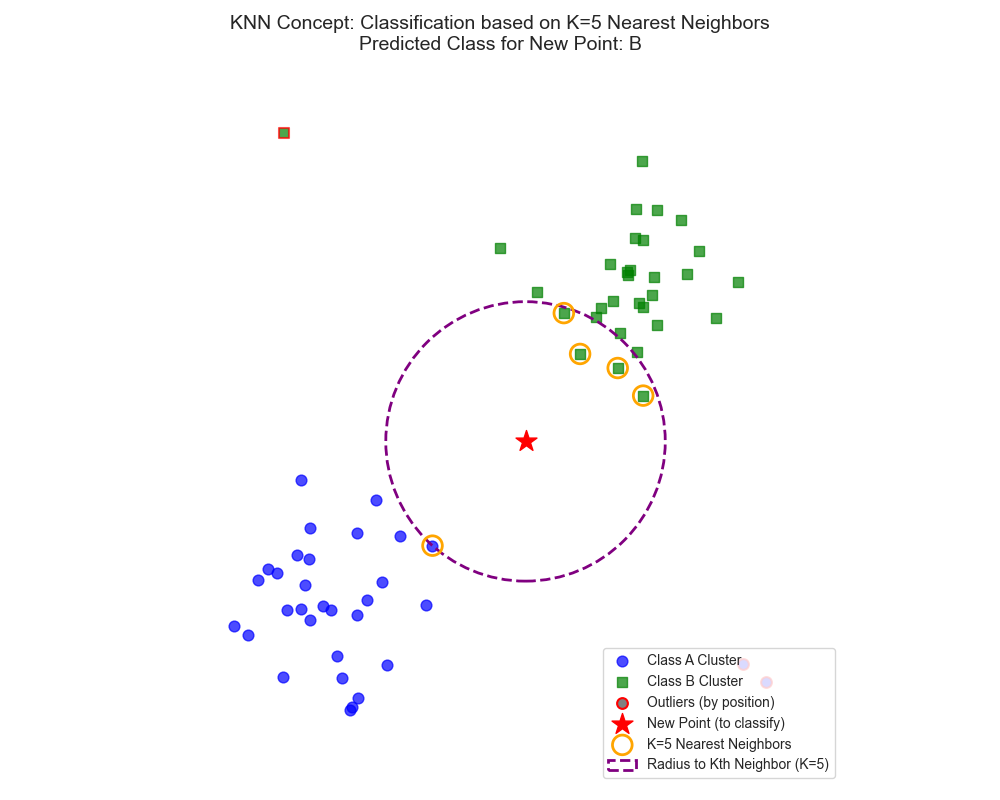
\includegraphics[width=0.8\textwidth]{figures/knn.png}
  \caption[KNN Intuition]{KNN algorithm. The algorithm classifies a new data point based on the majority class of its $K$ nearest neighbours in the training dataset. Euclidean distance metric has been used to determine the distance between data points.}
  \label{fig:knn}
  \caption*{Own illustration.}
\end{figure}

In the given figure, the lazy learning approach of KNN near completion is shown. The star-formed point has to be assigned to class one or two. Based on the count of points in the near region of the unassigned point, the algorithm will decide class two.
The approach by \textcite{dos2024simulation} integrates KNN with p-charts for the concurrent validation of \gls{sbdt} \autocite{dos2024digital}. This involves monitoring the \gls{dt}s output over time and using KNN to classify its behaviour. Subsequently, p-charts are employed to statistically monitor the proportion of anomalies detected by KNN. The X-axis represents the discretized time $t$, the Y-axis represents the proportion of anomalies detected by the KNN. P-charts normally show a relative proportion of nonconforming items in a sample \autocite{acosta1999improved}. \Textcite{dos2024simulation} enriched their chart with an upper control limit (UCL) and lower control limit (LCL), which stand for acceptable statistical boundaries. This approach is similar to \textcite{Nie2023rcim} who also defined control intervals. If the p-value exceeds the boundaries, the twin may deviate from real behaviour. This method offers the advantage of real-time monitoring. However, it is sensitive to the choice of the hyperparameter $K$ and can be computationally expensive for large datasets \autocite{dos2024simulation}. The presence of outliers and noisy data can also impact the accuracy of KNN, and its performance may decrease in high-dimensional spaces. The authors utilized metrics such as accuracy, precision, recall and F1-Score, see \autoref{sec:metrics-theory}. They also used cross validation for increasing robustness of the prediction. By varying values for $K$, an optimal split may be found. Recalling the different kinds of anomalies from \autoref{sec:classification-methods}, KNN is able to capture point anomalies and contextual anomalies. Collective anomalies are not captured by KNN, as they are not able to learn from the data.

\begin{figure}[htbp]
  \centering
  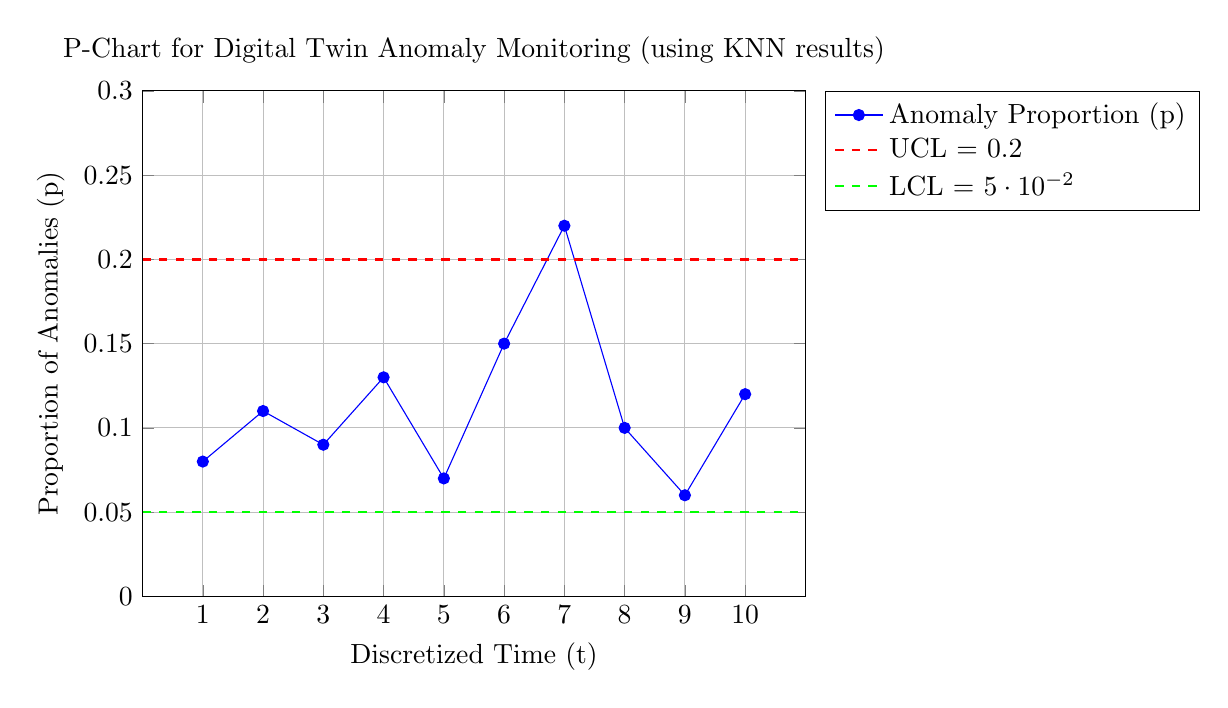
\begin{tikzpicture}
    % Define control limits (adjust values as needed for a real scenario)
    \def\ucl{0.20} % Upper Control Limit
    \def\lcl{0.05} % Lower Control Limit
    \def\cl{((\ucl)+(\lcl))/2} % Center Line (optional, average proportion)

    \begin{axis}[
        width=10cm, % Adjusted width
        height=8cm,  % Adjusted height
        grid=both,
        title={P-Chart for Digital Twin Anomaly Monitoring (using KNN results)},
        xlabel={Discretized Time (t)},
        ylabel={Proportion of Anomalies (p)},
        xmin=0, xmax=11, % Extend x-axis slightly beyond data
        ymin=0, ymax=0.3, % Adjust y-axis to fit data and limits
        xtick={1,2,3,4,5,6,7,8,9,10}, % Explicit ticks for discrete time
        yticklabel style={/pgf/number format/.cd,fixed,precision=2}, % Format y-labels
        scaled y ticks=false, % Show actual proportion values
        legend pos=outer north east, % Place legend outside
        legend cell align={left},
      ]

      % --- Simulated Data: Proportion of anomalies detected by KNN over time ---
      % Replace this with actual data if available
      % Format: (time_step, proportion)
      \addplot+[mark=*, blue, solid, mark options={fill=blue}]
      coordinates {
          (1, 0.08) % Time 1, 8% anomalies
          (2, 0.11) % Time 2, 11% anomalies
          (3, 0.09) % Time 3, 9% anomalies
          (4, 0.13) % Time 4, 13% anomalies
          (5, 0.07) % Time 5, 7% anomalies
          (6, 0.15) % Time 6, 15% anomalies
          (7, 0.22) % Time 7, 22% anomalies - Exceeds UCL!
          (8, 0.10) % Time 8, 10% anomalies
          (9, 0.06) % Time 9, 6% anomalies
          (10, 0.12)% Time 10, 12% anomalies
        };
      \addlegendentry{Anomaly Proportion (p)}

      % --- Control Limits ---
      % Upper Control Limit (UCL)
      \addplot[const plot, dashed, red, thick, domain=\pgfkeysvalueof{/pgfplots/xmin}:\pgfkeysvalueof{/pgfplots/xmax}] {\ucl};
      \addlegendentry{UCL = \pgfmathprintnumber{\ucl}}
      % Add label directly to the line (alternative to legend)
      % \node[anchor=west, red] at (axis cs:\pgfkeysvalueof{/pgfplots/xmax},\ucl) {UCL}; 

      % Lower Control Limit (LCL)
      \addplot[const plot, dashed, green, thick, domain=\pgfkeysvalueof{/pgfplots/xmin}:\pgfkeysvalueof{/pgfplots/xmax}] {\lcl};
      \addlegendentry{LCL = \pgfmathprintnumber{\lcl}}

    \end{axis}
  \end{tikzpicture}
  \caption[Proportion chart for VVUQ]{Example P-Chart showing the proportion of anomalies detected by KNN over time for \gls{dt} accreditation, with Upper (UCL) and Lower (LCL) control limits. A point outside the limits (like at t=7) suggests potential deviation.}
  \label{fig:pchart_knn_dt}
  \caption*{Own illustration based on \textcite{dos2024simulation}. \ai{AI generated based on copyrighted image.}}
\end{figure}

\subsubsection*{Time Series Classification for Fault Localization}
Time series classification techniques also play an important role in detecting and classifying anomalies within manufacturing \gls{dt} systems \autocite{Lugaresi2023compind}. These techniques involve training classifiers on simulation data generated by the \gls{dt} to identify and categorize faults in the real physical system \autocite{dihan2024digital}. A case study involving a scale-model gantry crane demonstrates the application of time series classification for this purpose \autocite{mertens2024localizing}.
Other techniques in this domain often involve deep learning models such as CNN, RNN, and LSTM networks. These models perform well at automatically extracting relevant features from time series data \autocite{cao2023real}, outperforming traditional rule-based or statistical methods in complex scenarios. Time series classification offers the benefits of automated anomaly detection and classification, with the potential for early fault prediction. However, a key challenge is the need for sufficient labelled data for training these models \autocite{zemskov2024security}, and real-time performance is often a critical requirement.

\subsubsection*{Uncertainty Quantification for Digital Twin Validation}
\label{sec:uq-dt}
V\&V is an important aspect of \gls{sbdt}, but uncertainty quantification (UQ) is equally crucial. UQ aims to quantify the uncertainty associated with the predictions made by the \gls{dt}, providing insights into the reliability and confidence of its outputs \autocite{sel2025survey}. Certainty in predictions creates trust in the application, a desirable property of \gls{sbdt} when used in practice \autocite{dwivedi2023explainable}. State of the art approaches to tackle uncertainty are Bayesian Neural Networks (BNN) \autocite{li2017dynamic}, Monte Carlo Dropout (MCD), Deep Ensembles (DE) and Gaussian Processes (GP). BNNs are able to quantify epistemic and aleatoric uncertainty (see \autoref{sec:uncertainty-quantification}. They are a type of neural network that introduce uncertainty into its predictions by treating the weights and biases as probability distributions rather than fixed values. Thus, each weight has a mean and a variance parameter for quantifying its uncertainty. During inference, samples are drawn from this distribution to \textit{learn} its characteristics. This allows the model to capture uncertainty in the data and make probabilistic predictions \autocite{li2017dynamic}. MCD, DE and GP train surrogate models (see \autoref{par:surrogate}) to approximate the uncertainty in the models predictions.

MCD is a technique that uses dropout \autocite{srivastava2014dropout} during both training and inference phases to approximate the uncertainty in the models predictions, unlike traditional dropout which is only used during training. By randomly dropping out neurons during inference with a chosen probability $p$, MCD generates multiple predictions, which then are averaged and can be used to estimate uncertainty. The key insight here is that effectively the sampling happens from a dozen different NN because of their different weight configurations. Thus, ensemble-learner like accuracy without the computational cost of training multiple complete models like in DE has been reached.
DE involves training multiple models with different initializations and architectures, and then combining their predictions to obtain a more robust estimate of uncertainty \autocite{rahaman2021uncertainty}. The difference between DE and MCD lies in statistically independent NNs, meaning they do not share statistical interaction processes. Furthermore, they are initialized randomly, whereas MCD networks share the same weight initialization. MCD and DE both provide good estimates for uncertainty, but it is recommended to apply both techniques after fine-tuning of the DNN architecture \autocite{kamali2024advancements}.
GPs are a non-parametric Bayesian approach that models the underlying function as a distribution over functions \autocite{bilionis2012multi}. They provide a measure of uncertainty in their predictions by estimating the variance and mean of the predicted outputs \autocite{Burr2025TEADT}.

Overall \gls{vvuq} for \gls{sbdt} is conducted with varying efforts. There is not a lot of research on fully automated \gls{vvuq} processes. The SLR by \textcite{Bitencourt2023} shows that most authors still rely on manual methods, if \gls{vvuq} has been performed at all. The trend towards more sophisticated \gls{dt}s and the increasing complexity of models will likely drive further research in this area. The SLR also highlights the need for more automated and standardized \gls{vvuq} processes, especially in the context of UQ. Very few authors performed fully automated \gls{vvuq} for \gls{dt}. The ones who did were presented in this section.

This chapter established the theoretical foundation for the thesis, focusing on \gls{sbdt}. It covered key concepts including the simulation of \gls{dmfs} using \gls{des}, and an analysis of different \gls{dt} architectures such as \gls{sbdt}, \gls{dddt}, and \gls{hdt}. The role of KPIs in balancing \gls{sbdt} trade-offs was described. \gls{pm}, particularly using \gls{ocel} for validation due to its ability to handle complex interactions, was explored. Furthermore, the chapter addressed \gls{vvuq}, contrasting traditional methods with modern ML approaches like KNN and BNN for ensuring \gls{sbdt} reliability. The need for automated \gls{vvuq} frameworks and associated challenges, like UQ, were highlighted. These theoretical elements underpin the development of the proposed \gls{sbdt} \gls{vvuq} framework aimed at enhancing reliability, which will be detailed in the next chapter.




